\documentclass[twoside]{article}

\usepackage{aistats2025}

% \usepackage{biblatex}
\usepackage{natbib}
\usepackage{amsmath,amssymb,amsthm}
\usepackage{graphicx}
\usepackage{subcaption}
\usepackage{xcolor}

\newcommand{\avg}{\mathrm{avg}}
\newcommand{\E}{\mathbb{E}}
\newcommand{\he}{\mathrm{he}}
\newcommand{\He}{\mathrm{He}}
\newtheorem{theorem}{Theorem}
\newtheorem{lemma}{Lemma}
\newtheorem{remark}{Remark}
\newtheorem{corollary}{Corollary}
\newtheorem{proposition}{Proposition}
\theoremstyle{definition}
\newtheorem{definition}{Definition}
% \newtheorem{corollary}[theorem]{Corollary}
\newcommand{\thomas}[1]{{\color{blue}TH:  \textit{#1}}}
\newcommand{\amir}[1]{{\color{cyan}AJ:  \textit{#1}}}
\graphicspath{ {./figures/} }


\begin{document}

% Title and authors
\twocolumn[
\aistatstitle{Emergence of Globally Attracting Fixed Points in Deep Neural Networks With Non-linear Activations}
\aistatsauthor{Anonymous Author(s)}
\aistatsaddress{Affiliation(s)} ]

\begin{abstract}
Understanding how neural networks transform input data across layers is fundamental to unraveling their learning and generalization capabilities. While prior work has leveraged insights from kernel methods to study neural networks, a global analysis of how the similarity between hidden representations evolves across layers remains underexplored. In this paper, we introduce a theoretical framework for the evolution of the kernel sequence, which measures similarity between hidden representation for two different inputs. Operating under the mean field regime, we show that the kernel sequence evolves deterministically via a kernel map, which only depends on the activation function. By expanding activation using Hermite polynomials and using their algebraic properties, we derive an explicit form for kernel map, and fully characterize its fixed points. Our analysis reveals that for non-linear activations, the kernel sequence converges globally to a unique fixed point, which can correspond to orthogonal or similar representations depending on the activation and network architecture. We further extend our results to networks with normalization layers, demonstrating similar convergence behaviors. This work provides new insights into the implicit biases of deep neural networks and how architectural choices influence the evolution of representations across layers.
\end{abstract}


% \section{Fixed-points and global convergence of deep representations}
% \label{ch:isometry_activation}

\section{Introduction}
The study of neural networks has increasingly focused on understanding the internal mechanisms that govern their learning and generalization capabilities. A central aspect of this inquiry is how neural networks transform and preserve input data structure as it passes through multiple layers. One powerful approach to studying these transformations is through the lens of kernel methods, which have long been used in machine learning to understand the relationships between data points in high-dimensional spaces \citep{scholkopf2002learning,smola2004tutorial}.

Analyzing neural networks from the perspective of kernels has been the subject of many theoretical studies. This perspective has led to significant advancements, most notably the Neural Tangent Kernel (NTK) introduced by \citet{jacot2018neural}, which provided a framework to analyze the training dynamics of infinitely wide neural networks. Additionally, Convolutional Kernel Networks by \citet{mairal2014convolutional} and the notion of dual kernels in \citet{daniely2016toward} have expanded our understanding of neural networks through kernel methods. The idea that neural networks, especially in the infinite-width limit, can be understood through the lens of kernels has been explored in various recent works~\citep{lee2019wide, arora2019exact, yang2019scaling}. Moreover, the use of kernel methods to measure the similarity between inputs as the network processes them provides a powerful means of understanding the inductive biases and representative capacity of neural networks, particularly in the context of deep learning (cf.~\citep{zhang2017understanding,zhang2021understanding,cho2009kernel}).

Despite this extensive line of research, the question of how the similarity between hidden layer representations evolves across layers and whether it converges globally to a fixed point remains an important but underexplored area of study. Previous works, such as \citet{saxe2013exact}, \citet{schoenholz2016deep}, and \citet{pennington2017resurrecting}, have analyzed signal propagation and dynamical isometry in deep networks, focusing on local behaviors and specific initialization conditions. However, a comprehensive global analysis of fixed points and convergence properties of kernel sequences, particularly in the presence of nonlinear activations, is still incomplete. Specifically, while previous research has provided insights into local behaviors (cf.~\citep{yang2019meanfield}), a global analysis of fixed points and convergence properties of kernel sequences, particularly in the presence of nonlinear activations is still incomplete.

This paper addresses this gap by introducing and analyzing the evolution of the kernel through layers. The kernel sequence tracks the similarity between two inputs. More concretely, we consider the kernel sequence $k(h^\ell(x), h^\ell(y)),$ where $k$ denotes some notion of similarity, such as inner product or cosine similarity, and $h^\ell(x)$ and $h^\ell(y)$ denote layer $\ell$ representation for respective inputs $x$ and $y$. Understanding whether and how this sequence converges to a fixed point as the network depth increases is crucial for uncovering the inherent implicit biases of deep networks.

Our analysis builds upon foundational work in understanding the role of activation functions in neural networks, such as the use of ReLU and its variants (cf.~\citep{glorot2011deep, nair2010rectified}) and the exploration of nonlinear activations in large-scale models by~\citep{ramachandran2017searching, clevert2015fast}. Additionally, the interplay between activation functions and normalization techniques, such as layer normalization (\citep{ba2016layer}), plays a critical role in shaping the convergence behavior of kernel sequences (\citep{klambauer2017self, hayou2019impact}). Moreover, the study of neural networks through the lens of kernel methods is deeply connected to earlier work by \citep{williams2006gaussian} on Gaussian processes and the dynamics of signal propagation in deep networks in \citep{poole2016exponential, raghu2017expressive}. By analyzing how these kernels evolve across layers, particularly in terms of activation functions, we contribute to a deeper understanding of the dynamics within deep neural networks.

Throughout this paper, we assume that the network operates under the mean field regime, which simplifies the analysis by considering the infinite-width limit and making stochastic sequences deterministic. This approach is inspired by prior studies that have employed mean field theory to analyze neural networks \citep{poole2016exponential, yang2019meanfield, mei2019mean}.
% \thomas{Would be good to provide a reference and explain a bit more. Not all readers may be familiar.}

\section{Related works}
The study of deep neural networks through the lens of kernel methods and mean field theory has garnered significant interest in recent years. Notably, the Neural Tangent Kernel (NTK) introduced by \citet{jacot2018neural} provided a framework to analyze the training dynamics of infinitely wide neural networks using kernel methods. This perspective was further expanded upon by \citet{lee2019wide} and \citet{arora2019exact}, who explored the connections between neural networks and Gaussian processes.

The propagation of signals in deep networks has been studied using mean field theory, as seen in the works of \citet{schoenholz2016deep} and \citet{pennington2017resurrecting}. These studies focused on understanding the conditions required for the stable propagation of information and the avoidance of signal amplification or attenuation. However, these analyses often concentrated on local behaviors or specific conditions, leaving a gap in understanding the global evolution of representations across layers.

Hermite polynomials have been employed in probability theory and statistics, particularly in the context of Gaussian processes \citep{williams2006gaussian}. While \citet{poole2016exponential} and \citet{daniely2016toward} have utilized polynomial expansions to analyze neural networks, the explicit use of Hermite polynomial expansions to derive kernel maps and analyze fixed-point dynamics in neural networks, as presented in this paper, is novel.

Our work extends these foundational studies by providing an explicit algebraic framework to analyze the global convergence of kernel sequences in deep networks with non-linear activations. By leveraging Hermite polynomial expansions, we offer a precise characterization of the kernel map and its fixed points, contributing new insights into the implicit biases and representational dynamics of deep neural networks.

\section{Preliminaries}
In this section, we introduce the fundamental concepts, notations, and definitions used throughout this paper. 
If $X$ and $Y$ are vectors in $\mathbb{R}^n$, we use the inner product notation $\langle X, Y \rangle_\avg$ to denote their average inner product $ = \frac{1}{n} \sum_{i=1}^n X_i Y_i,$ and analogously $\|X\|_\avg = \sqrt{\langle X, X \rangle_\avg}$ to denote mean norm, which is otherwise known as Root Mean Square (RMS) norm. 

% For scalar random variables $X$ and $Y,$ will use $\langle X, Y\rangle$ to denote the covariance $\langle X, Y \rangle = \E X Y.$ Furthermore, if $X$ and $Y$ are vectors of dimension $n$, we use the same notation to to denote averaged inner product $\langle X, Y\rangle = \frac{1}{n} X_i Y_i. $ The main reason for this notation is that if elements of $X$ and $Y$ are independent copies of some distribution, by law of large numbers we will have $\langle x, y\rangle = \frac1n \sum_{i=1}^n x_i y_i \to \E X Y = \rangle X,Y\rangle. $ 

We consider a feedforward neural network with $L$ layers and constant layer width $d$. The network takes an input vector $x \in \mathbb{R}^d$ and maps it to an output vector $h^L(x) \in \mathbb{R}^d$ through a series of transformations. The hidden representations at each layer $\ell$ are denoted by $h^\ell(x)$. The transformation at each layer is composed of a linear transformation followed by a nonlinear activation function $\phi$. Mathematically, the hidden representation at layer $\ell$ is given by:
\begin{align}
& h^\ell(x) = \phi\left(\frac{1}{\sqrt{d}}W^\ell h^{\ell-1}(x)\right), && W^\ell \in \mathbb{R}^{d \times d},
\end{align}
where $h^0(x)=x$ is identified with the input. We can assume elements of $W^\ell$ are assumed to be drawn i.i.d.~from a zero mean distribution, unit variance distribution. Two prominent choices for weights distributions, Gaussian $N(0,1)$ and uniform distribution $\text{Uniform}[-1,1],$ satisfy these conditions. In some variations of the MLP, we will use normalization layers to adjust the activations at each layer, namely Layer Normalization (LN) or Root Mean Squared (RMS) normalization. Finally, the neural kernel between two inputs $x$ and $y$ at layer $\ell$ is defined as:
\begin{align}
    \rho_\ell = \langle h^\ell(x), h^\ell(y) \rangle_\avg \,.
\end{align}
% where $\langle \cdot, \cdot \rangle$ denotes the inner product.
% and $\rho_0$ corresponds to similarity between input samples $x$ and $y$.

The main goal of this paper is to analyze the sequence $\{\rho_\ell\}$ at random initialization. The motivation for this analysis is to understand if architectural choices, specifically the activation function and the model depth, lead to specific biases of the kernel towards a certain fixed point. Namely, if there is a bias towards zero, it would imply that at initialization, the representations become more orthogonal. In contrast, a positive fixed point would mean the representations become more similar.

In the current setup, the sequence $\{\rho_\ell\}$ is a stochastic sequence or a Markov chain due to the random weights at each layer. However, we will show that under the mean field regime, the sequence $\{\rho_\ell\}$ converges to a deterministic sequence, and we will analyze its properties.


\section{Mean-field Regime}

In this section, we conduct a mean field analysis of multilayer perceptrons (MLPs) to explore the neural kernel's fixed-point behavior as the network depth increases. This approach allows us to gain insight into the global dynamics of neural networks, mainly how the similarity between two input samples evolves as they pass through successive network layers.
Now, we can state the mean field regime for the kernel sequence, stating that in this regime, the sequence becomes deterministic. 

As will be proven later, the deterministic transition of this sequence follows a scalar function that is defined below. 

\begin{definition}
    \label{def:kernel_map}
Given two random variables $X, Y$ with covariance $\rho,$ and activation $\phi,$ define the \emph{kernel map } $\kappa$ as the mapping between the covariance of pre-activations and the covariance of post-activations:
\begin{align}
& \kappa(\rho):=\mathbb{E}[\phi(X)\phi(Y)], && 
 X, Y\sim \mathcal N\left(0, \begin{pmatrix} 1 & \rho \\ \rho & 1 \end{pmatrix}
 \right)
 \label{eq:kernel_map}
\end{align}
% \thomas{I would suggest to use this notation for a joint normal distribution, unless you had  something else in mind.}
% \begin{align}
%     \kappa(\rho):=\E_{X,Y}[ \phi(X)\phi(Y)], && X, Y\sim N(0,1),\; \rho:=\E XY.
% \end{align}
\end{definition}

The following proposition formally states that in the mean field regime, the kernel sequence follows iterative applications of kernel map. 

\begin{proposition}
\label{prop:mean_field_kernel_general}
In the mean field regime with $d \to \infty$, let $\rho_\ell$ denote the kernel sequence of an MLP with activation function $\phi$ obeying $\E\phi(X)^2=1$ for $X\sim \mathcal N(0,1)$. If each element of the weights is drawn i.i.d.~from a distribution with zero mean and unit variance, the kernel sequence evolves deterministically as follows:
\begin{align*}
&\rho_{\ell+1} = \kappa(\rho_\ell),
\end{align*}
where the initial value $\rho_0$ corresponds to the input, and $\kappa$ is defined in Definition~\ref{def:kernel_map}. 
% \thomas{Changed this a bit. Original is in comment.}
% \begin{align*}
% &\rho_{\ell} = \mathbb{E}_{X,Y}[\phi(X)\phi(Y)], && 
%  X, Y\sim N(0,1),\; \E XY = \rho_{\ell-1}.
% \end{align*}
% where the initial value $\rho_0$ corresponds to the input. 

\end{proposition}


% Inspired by this property, we define the mapping between the covariance of pre-activations and the covariance of post-activations.
% \thomas{The English is a bit corrupted. Clarify, please.}

Historically, conditions similar to $\E \phi(X)^2=1$ have been used to prevent quantities on the forward pass from vanishing or exploding. For example, in a ReLU  half of the activations will be zeroed out, which will lead to a vanishing norm of forward representations. The initialization  of
\citep{he2016deep} addresses that by scaling weights to maintain consistent forward pass norms across layers. This principle is further refined in \citep{klambauer2017self} idea of self-normalizing activation functions, which ensure consistent mean and variances between pre- and post-activations. 

One interesting observation is that the kernel dynamics is governed by kernel map $\kappa,$ defined based on Gaussian pre-activations, even if the weights are not Gaussian matrices. The main insight for this equivalence is that as long as elements are drawn i.i.d.~from a zero mean unit variance distribution, we can apply Central Limit Theorem (CLT) to conclude that pre-activations follow the Gaussian distribution. This simple yet elegant observation gives us a very powerful tool to study kernel dynamics by leveraging algebraic properties for Gaussian pre-activations, and automatically get the same results for a wide class of distributions. 

Proposition~\ref{prop:mean_field_kernel_general} tells us that the sequence is given by $\rho_0,\kappa(\rho_0),\kappa(\kappa(\rho_0)),\dots\,.$ Thus, we can analyze its convergence by studying the fixed-points of the kernel map $\kappa,$
which are the values of $\rho^*$ that satisfy $\kappa(\rho^*) = \rho^*.$ 

With the assumption that $\E \phi(X)^2=1,$ the kernel map $\kappa$ is a mapping between $[-1,-1]$ to itself. Thus, Brower's fixed-point theorem implies that the kernel map $\kappa$ has at least one fixed point $\rho^*.$ But as we will show, there is potentially more than one fixed point, and it will be interesting to understand which ones are locally or globally attractive. 


\section{Hermite expansion of activation functions}
Hermite polynomials possess completeness and orthogonality under the Gaussian measure. Thus any function that is square-integrable with respect to a Gaussian measure can be expressed as a linear combination of Hermite polynomials (see below). The square integrability of activation functions avoids heavy-tailed post-activations with diverging second moment. It holds for all activations that are used in practice. We use the \emph{normalized} Hermite polynomials and their coefficients. 

\begin{definition}
Normalized Hermite polynomials $\he_k(x)$ are defined as follows
\begin{align*}
&\he_k(x) :=\frac{1}{\sqrt{k!}}(-1)^k e^{-\frac{x^2}{2}} \frac{d^k}{dx^k} e^{-\frac{x^2}{2}}.
\end{align*}
\end{definition}

While Hermite polynomials have been traditionally used in probability theory and statistics, particularly in the context of Gaussian processes \citep{williams2006gaussian}, their application in analyzing neural network dynamics provides a novel methodological tool. Previous works, such as \citet{daniely2016toward}, have utilized polynomial expansions to study neural networks, but our explicit use of Hermite polynomial expansions to derive the kernel map and analyze convergence is a new contribution.


% \thomas{Maybe we don't need a table object here...}
% Table~\ref{table:hermite_poly} shows the first few normalized Hermite polynomials.

% \begin{table}[ht]
%     \centering
%     \caption{Hermite polynomials and their normalized versions}\label{table:hermite_poly}
%     \begin{tabular}{|c|c|c|c|c|}
%     \hline
%  Order & $k=0$ & $k=1$ & $k=2$ & $k=3$  \\
%  \hline
%  % $\He_k(x)$ & $1$ & $x$ & $ (x^2 - 1)$ & $(x^3 - 3x)$  \\    
%  % \hline
%  $\he_k(x)$ & $1$ & $x$ & $\frac{1}{\sqrt{2}} (x^2 - 1)$ & $\frac{1}{\sqrt{6}} (x^3 - 3x)$ \\
%     \hline
%     \end{tabular}
% \end{table}

The crucial property of Hermite polynomials is their  orthogonality:
\begin{align}\label{eq:hermite_orthogonality}
\E\left[\he_k(X)\he_l(X)\right] = \delta_{kl}, \quad X \sim \mathcal N(0,1).
\end{align}
The scaling by $1/\sqrt{k!}$ ensures that polynomials form an \emph{orthonormal} basis.  Based on this property, we can define:
\begin{definition}\label{def:hermite_expansion}
Given a function $\phi$, square-integrable with respect to the Gaussian measure. Its Hermite expansion is given by:
\begin{align*}
\phi = \sum_{k=0}^\infty c_k \he_k,\; c_k = \E\left[\phi(X) \he_k(X)\right], \; X \sim \mathcal N (0,1)\,.
\end{align*}
Here $c_k$ are called the Hermite coefficients of $\phi$. 
\end{definition}

% Based on the orthogonality of Hermite polynomials, we can make a few observations about some of the Hermite coefficients.  

Besides orthogonality, Hermite polynomials have another `magical' property that is crucial for our later analysis. 

\begin{lemma}[Mehler's lemma]\label{lem:mehler_kernel}
For standard-normal random variables $X,Y$ with covariance $\rho$ it holds
\begin{align*}
\E\left[\he_k(X)\he_l(Y)\right] = \rho^n \delta_{kl}, && X, Y\sim \mathcal N\left(0, \begin{pmatrix} 1 & \rho \\ \rho & 1 \end{pmatrix}
 \right).
\end{align*}
\end{lemma}

This lemma states that given two Gaussian random variables $X, Y$ with covariance $\rho$, the expectation of the product of Hermite polynomials is zero unless the indices are equal. 
Lemma~\ref{lem:mehler_kernel} is crucial for our theory. Based on this lemma, we can express the kernel map $\kappa$ in terms of the Hermite coefficients, showing a particular structure of the kernel map.

\begin{corollary}
    \label{cor:hermite_covariance}
    \label{cor:kernel_map}
We have the following explicit form for kernel map:
\begin{align*}
\kappa(\rho) = \sum_{k=0}^\infty c_k^2 \rho^k.
\end{align*}
\end{corollary}
% thanks for the catch, you are right, it ought to be E phi(X)phi(Y) ... 
% \thomas{Something wrong in the corollary. What happened to $Y$? I guess its meant to be
% \begin{align*}
% \kappa(\rho) = \E\left[\phi(X)\phi(Y)\right] = \sum_{k=0}^\infty c_k^2 \rho^k.
% \end{align*}
% }

The proof follows directly from the definition of kernel map, expanding $\phi$ in the Hermite basis and then applying Lemma~\ref{lem:mehler_kernel}. 

% \begin{proof}[Proof of Corollary~\ref{cor:hermite_covariance}]
% Using Lemma~\ref{lem:mehler_kernel} we have
% \begin{align*}
% \E_{X\sim N(0,1)} &\left[\phi(X)\phi(X)\right] \\
% &= \E_{X\sim N(0,1)} \left[\sum_{k=0}^\infty c_k \he_k(X)\sum_{l=0}^\infty c_l \he_l(X)\right] \\
% &= \sum_{k=0}^\infty c_k^2 \rho^k.
% \end{align*}
% \end{proof}

These algebraic properteis of kernel map will be crucial in our analysis of the convergence of the kernel sequence to a fixed point. 

% Before we turn our attention to convergence, let us draw some links between the properties of activation functions, its kernel map, and its Hermite coefficients.
% \thomas{I am not sure I understand the table below. Does the first case include $\tanh$?}

% \begin{table}[ht]
% \small 
%     \centering
%     \caption{Properties of activations in terms of Hermite coefficients and kernel map: 1) centered, 2) stable, 3) non-linearity. }
%     \begin{tabular}{|c|c|c|c|}
%     \hline 
%  Prop & Activation $\phi$ & Coefs. $\{c_k\}_{k\ge 0}$ & Kernel map $\kappa$ \\
%     \hline
%  1 & $\E \phi(X)=0$ & $c_0 = 0$ & $\kappa(0) = 0$ \\
%     \hline
%  2 & $\E \phi(X)^2 = 1$ & $\sum_{k=0}^\infty c_k^2 = 1$ & $\kappa(1) = 1$ \\
%     \hline
%  3 & $\phi(x)$ nonlinear & $\sum_{k=2}^\infty c_k^2 > 0$ & $\kappa(\rho)$ nonlinear \\
%     \hline
%     \end{tabular}
% \end{table}



\section{Global attraction towards orthogonality for centered activations}

Recall that for activations that obey $\E \phi(X)^2 = 1$, the kernel map  $\kappa$ is a power series with non-negative coefficients $\sum_{k=0}^\infty c_k^2 \rho^k$ that maps $[-1,1]$ to itself, and obeys $\kappa(1)=1.$ This immediately reveals that $\rho=1$ is a fixed point of the kernel map. 
% This is unsurprising, as it reaffirms the fact that if two inputs are identical with unit variance, the post-activations will also be identical. \thomas{I find the term "identical" misleading. Same distribution?}  
However, it is far more interesting whether this fixed point is globally attractive and how the kernel map influences the convergence rate to this fixed point. In a similar vein, we can ask if there are other fixed points and how the kernel map influences the convergence rate to these fixed points.

In this section, we investigate properties in the kernel maps lead to convergence towards orthogonality. In other words, conditions that lead to $\rho^*=0$ being a fixed point, and whether this fixed point is globally attractive. \thomas{Maybe a few words of motivation why this is the most interesting case.}



% A quantity that will be crucial for our analysis is the contraction rate of the kernel map, which is defined based on the Hermite coefficients of the activation function.

% \begin{definition}
%     \label{def:contraction_rate}
%  Given activation $\phi$ that with Hermite coefficients $\{c_k\}_{k\ge 0},$ it contraction rate $\alpha$ is defined as:
%     \begin{align}\label{eq:contraction_rate}
%         \alpha = \frac{\sum_{k=1}^\infty c_k^2}{\sum_{k=1}^\infty  k c_k^2 } = \frac{\kappa(1)-\kappa(0)}{\kappa'(1)}.
%     \end{align}
% \end{definition}

% We can make the following important observation about the range and extreme values of the contraction rate $\alpha.$

% \begin{remark}
%     \label{rem:contraction_rate}
%  Note that the term 
%     $(\sum_{k=1}^\infty c_k^2)/(\sum_{k=1}^\infty k c_k^2)$
%  is always in the range $[0,1].$ Furthermore, $\alpha < 1$ if and only if the activation is non-linear, i.e., $c_k \neq 0$ for some $k\ge 2.$ We can also observe this from the second formulation: the numerator $(\kappa(1)-\kappa(0))/(1-0)$ encodes the slope of the line connecting $(0,\kappa(0))$ and $(1,\kappa(1)),$ and the denominator $\kappa'(1)$ is the slope of the tangent line at $\rho=1.$ Because $\kappa$ is convex in $[0,1]$ the tangent slope is higher than the line slope, which implies $\alpha\le 1,$ and it becomes strict if and only if the convexity is strict, i.e., the activation is non-linear. 
% \end{remark}


Finally, we can state one of the central results of this chapter, which characterizes the global convergence of the kernel map towards the fixed point $\rho^*=0.$

\begin{theorem}\label{thm:global_attract_centered}
Let $\phi$ be an activation function with kernel map $\kappa$ that is centered $\kappa(0)=0,$ and $\kappa(1)=1$. \thomas{So you are saying $\{0,1\}$ are fixed points, I guess?} Let $\rho_\ell$ be the kernel sequence generated by $\kappa$, given the initial value $\rho_0 \in(-1 , 1)$.
% \thomas{I think you need to exclude the non-stable fixed point. Added the inequality.} 
Then, the sequence contracts towards the fixed-point at zero $\rho^*=0$ with rate $\alpha$:
    \begin{align}
        &\frac{|\rho_\ell|}{1-|\rho_\ell|} \le \frac{|\rho_0|}{1-|\rho_0|}\alpha^{\ell}, && \alpha := \frac{1}{2-\kappa'(0)},
    \end{align}
 where $\alpha<1$ if the activation is non-linear. The only other fixed points can be $\rho^*=\pm 1$, and none of them is locally or globally attractive.
\end{theorem}

% Note that the statement becomes vacuous if the initial covariance is $\rho_0 = 1$ or $\rho_0 = -1$, as in these cases, the right-hand side goes to infinity, but the theorem is non-vacuous for all $\rho_0\in(-1,1).$ This is unsurprising, as the kernel map cannot separate the two inputs if they are identical or anti-identical. \thomas{I would restate. I would also simply exclude the boundary points from consideration to make the theorem above simpler. Maybe one can simple deal with the special cases in a corollarly.} In plain words, this states that if the two samples are not identical, by iteratively passing them through a nonlinear activation, the covariance between them will contract with rate $\alpha$ in expectation. \thomas{I would not say it like this. You are passing the inputs through a random ensemble and consider what happens in expectation.}  While it may not seem immediately obvious why $\alpha < 1$ for non-linear activations, the following remark makes the connection between the two.

% \begin{remark}
%     \label{rem:contraction_rate}
%     Let us assume $\kappa(\rho)=\sum_{k=0}^\infty c_k^2\rho^k,$ where $c_k$ denote Hermite coefficients. Note that $\kappa'(0) = c_1^2 \le \sum_{k=0}^\infty c_k^2 = \kappa(1)=1$. Now, if we have $\kappa'(1)=1,$ it implies that $c_k=0$ for all $k\ge 2.$ This is a contradiction with the assumption that the activation is non-linear.  
% \end{remark}
% \thomas{I am a bit lost of what the remark is trying to get at. Can you perhaps first add some remarks to why $\kappa'$ matters and what condition ensures stability or convergence. This is not quite clear.}

Another observation is that rather than proving convergence directly, we showed contraction under the potential $|\rho|/(1-|\rho|).$ Because $|\rho|/(1-|\rho|)$ is a monotonically increasing with $|\rho|$, the contraction of $|\rho_\ell|/(1-|\rho_\ell|)$ implies contraction of $|\rho_\ell|$ towards zero. 
While this form might look mysterious at first sight, there is an intuitive way of understanding why it occurs in our convergence formula. This insight comes from approximating our discrete dynamics in depth by a continuous time dynamical system. 

% \begin{corollary}
% Under the same setting as in Theorem~\ref{thm:global_attract}, the sequence $\rho_\ell = \kappa(\rho_{\ell-1})$ converges to zero with rate $|\rho_\ell| \le \rho_0/(1-|\rho_0|) \alpha^{\ell}$.
% \end{corollary}

% The proof follows directly from Theorem~\ref{thm:global_attract} and the inequality $|\rho_\ell| \le |\rho_\ell|\le (1-|\rho_\ell|).$ 


% We can now state and prove the main theorem of this section, which characterizes the global convergence of the kernel map towards the fixed point $\rho^*=0.$

% \begin{theorem}\label{thm:global_attract}
%  Consider activation $\phi,$ that with Gaussian pre-activations, has zero mean $\E_{X}\phi(X)=0$ and unit variance $\E_{X}\phi(X)^2 = 1,$ the sequence $\rho_\ell = \kappa(\rho_{\ell-1})$ contracts towards zero with rate $\alpha$:
%     \begin{align}
%         \Psi(\rho_\ell)\le \Psi(\rho_0) \alpha^{\ell}, 
%     \end{align}
%  where $\alpha$ is defined in \eqref{eq:contraction_rate}, which becomes strictly less than one if the activation is non-linear. 
% \end{theorem}

\subsection*{A continuous time differential equation approximation to the kernel dynamics} 
One of the most helpful ways to find insights into discrete fixed point iterations is to cast them as a continuous problem. More specifically, consider our fixed point iteration: 
\begin{align*}
    % \rho_{\ell+1} &= \kappa(\rho_\ell) = \sum_{k=1}^\infty c_k^2 \rho^k,\\
    \Delta \rho_\ell &= \rho_{\ell+1} - \rho_\ell = - \rho_\ell + \sum_{k=0}^\infty c_k^2 \rho^k_\ell.
\end{align*}
We can replace this discrete iterations by a continuous time differential equation, which we will refer to as the kernel ODE:
\begin{align}\tag{kernel ODE}\label{eq:kernel_ODE}
    d\rho/dt = -\rho + \sum_{k=0}^\infty c_k^2 \rho^k,
\end{align}
which we will refer to as the kernel ordinary differential equation (ODE). In most scenarios, kernel ODE will capture most important parts of the discrete kernel dynamics.  The continuous analogue of fixed points is a $\rho^*$ that satisfies $\rho'(\rho^*) = 0.$ Furthermore, the fixed point is globally attracting if we have $\rho'$ becomes negative for $\rho>\rho^*$ and positive for $\rho<\rho^*.$ We can say the fixed point is locally attracting if this property only holds in some small neighborhood of $\rho^*.$

While the kernel ODE presents an interesting transformation of the problem, it does not have a closed form solution in its general form. However, our main strategy is to find worst case (slowest) scenarios for convergence that correspond to tractable ODEs. In many cases however, the worst case scenario depends on some boundary conditions. Thus, we can design worst case ODE for different cases and combine them in a joint bound. Let us use our centered activation equation as a case study. 

\subsection*{Kernel ODE for centered activations}
For the case of centered activation in Theorem~\ref{thm:global_attract_centered}, the kernel ODE is given by
\begin{align*}
    \rho' = -(1-c_1^2)\rho + \sum_{k=2}^\infty c_k^2\rho^k\,,
\end{align*}
where the first term $k=0$ is canceled due to the assumption $\kappa(0)=c_0^2 = 1.$ 

Observe that $\rho'<0$ when $\rho>0,$ and $\rho'>0$ when $\rho<0.$ This implies that $\rho(t) \to 0$ for sufficiently large $t.$ Intuitively, the terms in $\rho'$ that have the opposite sign of $\rho,$ contribute to a faster convergence, while terms with a similar sign contribute to a slower convergence. Thus, we can ask what distribution of Hermite coefficients $\{c_k\}$ corresponds to the worst case, slowest convergence. If this is a tractable case, we can use its solution to bound the convergence of the original ODE. 

\textit{Positive range.}
Let us first consider the dynamics when $\rho\ge 0.$ 
In this case term corresponding to $k=1$ contribute positively to a faster convergence, while terms $k\ge 2$ make convergence slower. In light of this observation, a worst case (slowest possible) convergence rate happens when the positive terms are maximized, which occurs when the weight of all $\sum_{k=2}^\infty c_k^2 $ is concentrated on the $k=2$ term. \thomas{That makes sense. What is the worst case $\phi$? Does it make sense to state this for better illustration?}
\begin{align*}
    \frac{d\rho}{dt} &=  -(1-c_1^2)\rho + (1-c_1^2) \rho^2.
    % \\
    % &= -(1-c_1^2) \rho(1-\rho).
\end{align*}
where we used the fact that $\sum_{k=1}^\infty c_k^2 = 1.$ Intuitively, this means that the slowest convergence happens when $\phi$ is weighted average of first and second Hermite polynomials $\phi(x) = \beta \he_1 (x) + (1-\beta) \he_2 (x).$
% \thomas{You mean the sum equals $1$?} 
and thus $\sum_{k=2}^\infty c_k^2 = 1-c_1^2. $ Finally, we can solve this differential equation to get
\begin{align*}
    &\int \frac{d\rho}{\rho(1-\rho)} = - (1-c_1^2)\int t \\
    % \implies \ln \frac{|\rho(t)|}{|1-\rho(t)|} = -t (1-c_1^2) + C\\
    \implies &\frac{|\rho(t)|}{|1-\rho(t)|} = C \exp(-t(1-c_1^2)),
\end{align*}
where $C$ corresponds to the initial values. 
% Solving for the constant and assuming that our continuous approximation of the discrete equation is accurate, we can state that approximately:
% \begin{align*}
% \ln \frac{|\rho_\ell|}{|1-\rho_\ell|} =  \ln \frac{|\rho_0|}{|1-\rho_0|} -(1-\kappa'(0))\ell,
% \end{align*}
% where we removed absolute values around $1-\rho_\ell$ and $1-\rho_0$ because $\rho_\ell\le 1$ for all $\ell.$
% Observe that this is largely equivalent to the exact bound found in Theorem~\ref{thm:global_attract_centered}. 
% % \thomas{Is it safe to drop the absolute values around the $\rho_\ell$'s? You had them before.} 


\textit{Negative range.}
Now let us assume $\rho<0.$ In this case, only the odd terms in $\sum_{k=2}^\infty c_k^2 \rho^k$ contribute to a slowdown in convergence. Thus, the worst case occurs when all the weight of coefficients is concentrated in $k=3,$ corresponding to kernel equation 
\begin{align*}
&\frac{d\rho}{dt} = -(1-c_1^2)\rho + (1-c_1^2) \rho^3\\
\implies    &\int \frac{d\rho}{\rho(1-\rho^2)} = -(1-c_1^2)\int dt \\
% \implies \ln\left(\frac{|\rho(t)|}{\sqrt{1-\rho^2(t)}}\right) = - t (1-c_1^2) + B\\
\implies &\frac{|\rho(t)|}{\sqrt{1-\rho^2(t)}} = C' \exp(-t(1-c_1^2)),
\end{align*}
where $C'$ corresponds to the initial values. 

To summarize, we have obtained:
\begin{align*}
    \begin{cases}
        \frac{|\rho(t)|}{1-\rho(t)} \le C \exp(-\ell(1-c_1^2)) & \rho_0 \ge 0\\
        \frac{|\rho(t)|}{\sqrt{1-\rho(t)^2}}\le C' \exp(-\ell(1-c_1^2)) & \rho_0 < 0.
    \end{cases}
\end{align*}
Now, we can use a numerical inequality $\sqrt{1-x^2} \ge 1-|x|$ valid for all $x\in(-1,1),$ and by solving for the constant, we can construct a joint bound for both cases:
\begin{align*}
    \frac{|\rho(t)|}{1-|\rho(t)|} \le \frac{|\rho_0|}{1-|\rho_0|} \exp(-t (1-\kappa'(0))), 
\end{align*}
where we have also replaced $c_1^2=\kappa'(1).$  

We can observe that the kernel ODE rate derived by analysis of kernel ODE is largely aligned exponential convergence of this term in Theorem~\ref{thm:global_attract_centered}. The slight discrepancy between the exponential rates between Theorem~\ref{thm:global_attract_centered} and the kernel ODE rate $\exp(-(1-\kappa'(0))$ is due to the discrete-continuous approximation. 

It might be worth noting what activations correspond to the slowest convergence in positive and negative cases. In the positive case, any weighted average of first and second Hermite polynomials corresponds to the worst case $\phi = \beta \he_1 + (1-\beta) \he_2,$ for some $\beta \in(0,1),$ while in the negative case a weighted average of first and third Hermite polynomials corresponds to the slowest convergence $\phi = \beta \he_1 + (1-\beta)\he_3. $  

\begin{remark}
   The kernel ODE perspective reveals two important insights. 
   First, the appearance of $|\rho|/(1-|\rho|)$ formula in our bound is due to the fact that $x/(1-x) = \exp( -c t) $ is a fundamental solution of the differential equation $x' = - c x(1-x).$ Second, it reveals the importance of positivity of coefficients in $\sum_{k=0}^\infty c_k^2\rho^k,$ which allowed us to arrive at a worst case pattern for the coefficients. This further highlights the value of algebraic properties of Hermite polynomials that cancelled out the cross term in the kernel map. 
\end{remark}

% The main proof idea of this theorem is to show that upon applying the kernel map $\kappa$ to the covariance of pre-activations, the potential function $|\rho|/(1-|\rho|)$ decreases with rate $\alpha,$ and applying an induction over $\ell.$ Condition $\kappa(1)=\E \phi(X)^2 = 1$ ensures that activations are stable and do not explode or vanish, allowing us to apply the single step contraction inductively. The proof of the single step follows from the properties of Hermite polynomials and the orthogonality of the kernel map. The non-linearity condition is essential to have $\alpha<1,$ which rules out identity-like activations that do not change the value. The centered condition $\kappa(0)=\E \phi(X) = 0$ ensures that $\rho^*$ is a fixed point.

% Similar to before, we can use the fact that $\ln(x/\sqrt{1-x})=c dt$ is a fundamental solution to equation $x' = c x(1-x^2), $ to approximate the kernel dynamics:
% \begin{align*}
%     \ln\left(\frac{|\rho_\ell |}{\sqrt{1-\rho^2_\ell }}\right) - \ln\left(\frac{|\rho_0 |}{\sqrt{1-\rho^2_0 }}\right) = - t (1-c_1^2) \, .
% \end{align*}
% This corresponds to an activation that can be written as weighted average of first and third Hermite polynomials $\phi(x) = \beta \he_1(x) + (1-\beta) \he_3(x),$ for some $\beta\in(0,1).$ 
% \thomas{I think the conveying this insight is really helpful! Could profit from a little bit more of extra work to increase clarity.}
% 

% Some activations, such as SeLU~\citep{klambauer2017self}, which is a self-normalizing activation function that has $\E \phi(X)^1 = 0.$ 




\section{Convergence of the kernel with general activations}
So far, we only discussed the convergence of the kernel map for activations that are centered and the convergence of their kernel sequence towards zero. However, we can extend this analysis to general activations that are not centered. In this section, we will show that for any activation function that is non-linear, there is a unique fixed point $\rho^*$ that is globally attractive.


\begin{theorem}
\label{thm:global_attract}
Given a non-linear activation function $\phi$ with kernel  $\kappa$ such that $\kappa(1)=1$. Define the kernel sequence $\rho_{\ell+1}=\kappa(\rho_\ell)$, with  $\rho_0 \in (-1,1)$. Then there is a unique globally contracting fixed point $\rho^*$, which is necessarily non-negative $\rho^*\in[0,1]$. The only other fixed-points distinct from $\rho^*,$ could be $-1$ or $1,$ neither of which are locally or globally contracting \thomas{Maybe: neither of which is stable?}. Furthermore, we have the following contraction rate towards $\rho^*$:
\begin{enumerate}
    \item If $\kappa(0)=0$ then $\rho^*=0$ is an attracting with rate 
    \begin{align*}
    \frac{|\rho_\ell|}{1-|\rho_\ell|} \le \frac{|\rho_0|}{1-|\rho_0|} \alpha^\ell, && \alpha:=\frac{1}{2-\kappa'(0)}.
    \end{align*}
    \thomas{You introduced $\Phi$ above. Maybe one should use it here or not use the shortcut at all.}
    \item If $\kappa(0)>0$ and $\kappa'(1)<1$, then $\rho^*=1$ is attracting, with rate 
    \begin{align*}
    |\rho_\ell-1| \le |\rho_0-1| \alpha ^\ell, && \alpha := \kappa'(1).
    \end{align*}
    \item If $\kappa(0) > 0$, and $\kappa'(1)=1$ then  $\rho^*=1$ is attracting with rate 
    \begin{align*}
    |\rho_\ell-1| \le \frac{|\rho_0-1|}{\ell\alpha|\rho_0-1|+1}, && \alpha = 1-\kappa(0)-\kappa'(0).
    \end{align*}
    \item If $\kappa(0) > 0$, and $\kappa'(1)>1$ then the attracting fixed point is necessarily in the range $\rho^*\in(0,1)$, satisfying $\kappa'(\rho^*)\le 1,$ for which we have  
    \begin{align*}
    &|\rho_\ell-\rho^*| \le \frac{|\rho_0-\rho^*|}{1-|\rho_0|}\alpha^\ell \\ &\alpha = \max\left\{1-\kappa(0),\kappa'(\rho^*),\frac{1-\rho^*}{2-\kappa'(\rho^*)}\right\},
    \end{align*}
    where $\alpha<1$.
    % \thomas{I have dropped the `if is non-linear' and simply restricted to non-linear activations from the start. Hope that is ok.}
\end{enumerate}
\end{theorem}

\begin{remark}
One of the most striking results of this theorem is that for any non-linear activation, there is exactly one fixed point $\rho^*$ that is globally attractive, while other fixed points are neither globally or locally. 
\thomas{Well, there can only be one globally attractive fixed point, can't there, by definition?} 
\amir{Well, there is a possibility that there are multiple locally attracting fixed points, for example there are $\rho_1$ and $\rho_2$ and in the neighborhood of $\rho_1$, points are attracted towards $\rho_1$ and otherwise $\rho_2$. That is why the fact that any activation has exactly one globally attracting fixed points is quite interesting. Does it sound interesting now? }
Furthermore, the fixed point is necessarily non-negative. This implies that for any MLP with non-linear activations, the covariance of pre-activations will converge towards a fixed point, which is always non-negative. 
\thomas{Yeah, it seems that sign alternations can never reach a fixed-point, unless at $0$. Maybe this can just be excluded by a simple argument beforehand. I generally like to prune the space of possibilities early on. At any rate, a discussion of the special case of $\kappa$ taking negative values would probably be valuable.}
\end{remark}

\begin{remark}
    Let us take a step back and review the main take way from Theorem~\ref{thm:global_attract}. Omitting the constants and for sufficiently large depth $\ell,$ we have 
    \begin{align*}
        \langle h^{\ell}(x), h^{\ell}(y)\rangle_\avg =  \begin{cases}
             \rho^* + O(\alpha ^ \ell \langle x, y \rangle_\avg)  & \text{cases 1,2,4}\\
             \rho^* + O \left(\langle x, y \rangle_\avg/\ell \right)   & \text{cases 3}.
        \end{cases}
    \end{align*}
    Thus, an alternative way of viewing the statement of Theorem~\ref{thm:global_attract} is that, the bias of activations towards a global fixed points makes them forget about the similarity between two inputs exponentially in cases 1,2, and 4, and inversely in case 3.  
\end{remark}

% \begin{remark}
% The assumptions laid out in the theorem are nearly tight. For example, the non-linearity assumption is necessary to rule out identity activation, where every point in $[-1,1]$ is a fixed point. Furthermore, considering odd activations such as $\phi(x) = x^3,$ and we can see that if $\rho_0\in\{-1,1\}$, the sequence will remain the same $\rho_\ell=\rho_0,$ and hence will not converge, which implies the condition that $\rho_0\in(-1,1)$ is necessary. 
% \end{remark}

% \begin{remark}
% Note that the convergence rates are of exponential form $\|\rho_\ell-\rho^*\|= O(\alpha^\ell),$ where $\alpha<1$ if the activation is non-linear, with the exception of the case where $\kappa'(1)=1,$ where the rate is of the form $O(1/\ell).$ 
% \end{remark}

\section{Considering normalization and residual layers}

In this section, we will provide the statement and proof of two additional results considering normalization layers and skip connections. To state these results, let us consider some variants of the MLP with normalization layers and residual or skip connections. 

We consider two types of normalization layers, with normalization layers before or after the activation: 
\begin{align*}
    & \text{Pre-act norm: } &&h^\ell = \phi\left(\text{norm}\left(W^\ell h^{\ell-1}\right)\right), \\
    & \text{Post-act norm: } &&h^\ell = \text{norm}\left(\phi\left(W^\ell h^{\ell-1}\right)\right), 
\end{align*}
where $\text{norm}$ can be Layer Normalization (LN) or Root Mean Squared (RMS) normalization, defined as:
\begin{align*}
    &\text{LN}(z) = \frac{z - \bar{z}}{\sqrt{\frac1d \sum_{i=1}^d (z_i - \bar{z})^2}}, \\
    &\text{RMS}(z) = \frac{z}{\sqrt{\frac1d \sum_{i=1}^d z_i^2}}.
\end{align*}

For residual connections, we consider an update rule given by 
\begin{align*}
    h^\ell := \sqrt{1-r^2} \phi\left(\frac{1}{\sqrt{d}}W^\ell h^{\ell-1}\right) + r \frac{1}{\sqrt{d}}P^{\ell} h^{\ell-1}, 
\end{align*}
where $P^{\ell}\in R^{d\times d}$ are skip connections whose elements are drawn i.i.d.~from a zero mean unit variance distribution, and $r$ is the strength of the residual connections, the higher $r$ indicating stronger residual connections.   

\begin{theorem}
\label{thm:global_attract_res}
Consider an MLP with non-linear activation $\phi$ that obeys $\E_{X\sim N(0,1)} \phi(X)^2 = 1,$  with kernel map $\kappa(\rho),$ and residual strength $r.$ Let $\rho_\ell$ denote the kernel sequence of this MLP. Then, the kernel map of the residual MLP is given by 
\begin{align*}
    \nu(\rho) = (1-r^2) \kappa(\rho) + r^2 \rho.
\end{align*}
Furthermore, the new kernel map $\nu$ has the same globally contracting fixed point $\rho^*$ as the original kernel map $\kappa.$ Furthermore, if $r\in(0,1),$ the convergence case of $\nu$ remains in the same case  as $\kappa,$ but its convergence rate will be in each case. 
\end{theorem}

Theorem~\ref{thm:global_attract_res} reveals an intriguing property of skip connections, in that they do not alter the fixed points of the network, however, they may change the convergence behavior. It is rather remarkable that in all cases, the convergence speed strictly decreases with the strength of residual connections. f

Finally, we can state and prove the globally attracting fixed points for MLPs with the normalization layers.

\begin{theorem}
\label{thm:global_attract_norm}
Consider $\phi$ that is square-integrable $\E \phi(X)^2 =1,$ with kernel map $\kappa(\rho).$ We have 
\begin{itemize}
\item MLP with activation $\phi,$ pre-act RMS, post-act RMS, pre-act LN: The kernel sequence $\rho_\ell$ obeys by modified  kernel map $\kappa.$ 
% \begin{align*}
%     \nu(\rho):= \kappa(\rho)/\kappa(1).
% \end{align*}
\item MLP with post-act LN: The kernel sequence is defined by modified  kernel map $\nu$ 
\begin{align*}
    \nu(\rho) = \frac{\kappa(\rho)-\kappa(0)}{\kappa(1)-\kappa(0)}
\end{align*}
\end{itemize}
% the following contraction holds in the mean field regime:
% \begin{align}
%     &\frac{|\rho_\ell|}{1-|\rho_\ell|} \le  \frac{|\rho_0|}{1-|\rho_0|} \alpha^{\ell}, && \alpha = \frac{\kappa(1)-\kappa(0)}{\kappa'(1)}.
% \end{align}
% where $\alpha$ is strictly less than one if the activation is non-linear.
\end{theorem}

% \begin{remark}
%     Theorem~\ref{thm:global_attract_norm} states that if an activation obeys $\E \phi(X)^2 =1,$ from the standpoint of kernel convergence, the 
% \end{remark}


\section{Discussion}



The power of deep neural networks fundamentally arises from their depth and non-linearity. Despite substantial empirical evidence demonstrating the importance of deep, non-linear models, a rigorous theoretical understanding of how they operate and learn remains a significant challenge. Much of classical mathematical and statistical machinery was developed for linear systems or shallow models \citep{hastie2009elements}, and extending these tools to deep, non-linear architectures poses substantial difficulties. Our work takes a natural first step into this theoretical mystery by providing a rigorous analysis of feedforward networks with non-linear activations. 

By focusing on the algebraic patterns that emerge from viewing activations in the Hermite basis, we uncover several strikingly elegant properties inherent in non-linear activations. Our approach contrasts with traditional calculus-based methods that often involve complex and non-intuitive calculations. By leveraging mathematical patterns and symmetries inherent in Hermite polynomials, we provide a simpler and more concise framework. This perspective deepens our theoretical understanding shows avenues to demystify the inner workings of deep neural networks \citep{goodfellow2016deep, lecun2015deep}.


% Understanding the internal mechanisms of deep neural networks is a central challenge in machine learning. In this paper, we developed a theoretical framework to analyze the \emph{global} evolution of the kernel sequence in deep neural networks, focusing on its deterministic behavior in the mean field regime. By expanding activation functions using Hermite polynomials and leveraging their algebraic properties, we derived an explicit form for the kernel map and fully characterized its fixed points. Our analysis revealed that, for non-linear activations, the kernel sequence converges globally to a unique fixed point, which can correspond to orthogonal or similar representations depending on the activation function and network architecture.

One of the key contributions of our work is the global perspective in analyzing neural networks. Traditional analyses often focus on local structure, such as Jacobian eigenspectrum by \citet{pennington2018emergence}. While these local studies provide many  valuable insights, they do not capture the global kernel dynamics. However, real world inputs to neural networks, such as images of a dog and a cat, are not close enough to each other to be captured in the local changes. Our global approach allows us to study the evolution of representations across layers for any pair of inputs, providing further insights into how deep networks transform inputs with varying degrees of similarity.

% The power of deep neural networks fundamentally arises from their depth and non-linearity. Despite substantial empirical evidence demonstrating the importance of deep, non-linear models \citep{lecun2015deep, goodfellow2016deep}, a rigorous theoretical understanding of how they operate and learn remains a significant challenge. Much of classical mathematical and statistical machinery was developed for linear systems or shallow models \citep{hastie2009elements}, and extending these tools to deep, non-linear architectures poses substantial difficulties. Our work takes a natural first step into this theoretical mystery by providing a rigorous analysis of feed-forward networks with non-linear activations. By focusing on the algebraic patterns that emerge from viewing activations in the Hermite basis, we uncover several strikingly elegant properties inherent in non-linear activations.

% Our entirely \emph{algebraic} approach contrasts with traditional calculus-based methods that often involve complex integrations and differential equations. By relying on mathematical patterns and symmetries inherent in Hermite polynomials, our method is simpler and more concise, providing profound insights into the global dynamics of deep neural networks. This algebraic perspective not only deepens our theoretical understanding but also offers practical guidance for designing new architectures. Specifically, our findings illuminate how choices of activation functions, normalization techniques, and residual connections impact the evolution of representations across layers.

However, several limitations and avenues for future research remain. One interesting direction is to explore other global dynamics, such as the dynamics of norms in the absence of normalization layers. Without normalization, activations at each layer may deviate from the mean field assumptions, raising questions about the local and global dynamics of such deviations. Understanding these dynamics could provide deeper insights into how networks maintain stability and propagate information through layers.

While our results avoid complex calculus, this comes at the cost of not capturing finite-width discrepancies. Investigating the differences between finite-width and infinite-width results remains an important avenue for future work. Quantifying the exact discrepancies between limited-width and infinite-width scenarios, especially in the context of the Central Limit Theorem applied to pre-activations, would deepen our understanding of practical neural networks.

Another intriguing aspect is the potential for our work to inform the development of self-normalizing activation functions. Understanding the biases of different activation functions regarding stability and other properties could lead to a theory of self-normalizing activations \citep{klambauer2017self}, which aim to maintain mean and variance properties throughout the network layers without explicit normalization.

Furthermore, while the kernel is inherently tied to training dynamics, studying gradients and their structure—and how they relate to the mathematical foundations laid here—remains a highly interesting topic. Exploring first and second-order derivatives could provide deeper insights into optimization landscapes and training dynamics.

Our proof techniques for residual and normalization layers relied on several equivalences, such as replacing normalization layers with simple scalings and residual connections with an averaging of linear components. While these equivalences hold in the mean field kernel dynamics we studied, it would be valuable to investigate whether they remain valid during training and what other consequences they may have. This observation suggests the possibility of extending our algebraic approach to other architectures, such as convolutional neural networks and transformers, potentially offering new avenues for theoretical exploration in these domains.

In conclusion, our algebraic approach provides a new lens through which to understand the global dynamics of deep neural networks. By leveraging mathematical patterns and symmetries, we have gained profound insights into the evolution of representations and the impact of architectural choices. We hope that this work paves the way for further exploration into the mathematical foundations of deep learning and informs the design of more effective neural network architectures.

\bibliographystyle{plainnat}
\bibliography{refs}


\onecolumn

\section*{Checklist}


% %%% BEGIN INSTRUCTIONS %%%
The checklist follows the references. For each question, choose your answer from the three possible options: Yes, No, Not Applicable.  You are encouraged to include a justification to your answer, either by referencing the appropriate section of your paper or providing a brief inline description (1-2 sentences). 
Please do not modify the questions.  Note that the Checklist section does not count towards the page limit. Not including the checklist in the first submission won't result in desk rejection, although in such case we will ask you to upload it during the author response period and include it in camera ready (if accepted).

\textbf{In your paper, please delete this instructions block and only keep the Checklist section heading above along with the questions/answers below.}
% %%% END INSTRUCTIONS %%%


 \begin{enumerate}


 \item For all models and algorithms presented, check if you include:
 \begin{enumerate}
   \item A clear description of the mathematical setting, assumptions, algorithm, and/or model. [Yes/No/Not Applicable]
   \item An analysis of the properties and complexity (time, space, sample size) of any algorithm. [Yes/No/Not Applicable]
   \item (Optional) Anonymized source code, with specification of all dependencies, including external libraries. [Yes/No/Not Applicable]
 \end{enumerate}


 \item For any theoretical claim, check if you include:
 \begin{enumerate}
   \item Statements of the full set of assumptions of all theoretical results. [Yes/No/Not Applicable]
   \item Complete proofs of all theoretical results. [Yes/No/Not Applicable]
   \item Clear explanations of any assumptions. [Yes/No/Not Applicable]     
 \end{enumerate}


 \item For all figures and tables that present empirical results, check if you include:
 \begin{enumerate}
   \item The code, data, and instructions needed to reproduce the main experimental results (either in the supplemental material or as a URL). [Yes/No/Not Applicable]
   \item All the training details (e.g., data splits, hyperparameters, how they were chosen). [Yes/No/Not Applicable]
         \item A clear definition of the specific measure or statistics and error bars (e.g., with respect to the random seed after running experiments multiple times). [Yes/No/Not Applicable]
         \item A description of the computing infrastructure used. (e.g., type of GPUs, internal cluster, or cloud provider). [Yes/No/Not Applicable]
 \end{enumerate}

 \item If you are using existing assets (e.g., code, data, models) or curating/releasing new assets, check if you include:
 \begin{enumerate}
   \item Citations of the creator If your work uses existing assets. [Yes/No/Not Applicable]
   \item The license information of the assets, if applicable. [Yes/No/Not Applicable]
   \item New assets either in the supplemental material or as a URL, if applicable. [Yes/No/Not Applicable]
   \item Information about consent from data providers/curators. [Yes/No/Not Applicable]
   \item Discussion of sensible content if applicable, e.g., personally identifiable information or offensive content. [Yes/No/Not Applicable]
 \end{enumerate}

 \item If you used crowdsourcing or conducted research with human subjects, check if you include:
 \begin{enumerate}
   \item The full text of instructions given to participants and screenshots. [Yes/No/Not Applicable]
   \item Descriptions of potential participant risks, with links to Institutional Review Board (IRB) approvals if applicable. [Yes/No/Not Applicable]
   \item The estimated hourly wage paid to participants and the total amount spent on participant compensation. [Yes/No/Not Applicable]
 \end{enumerate}

 \end{enumerate}




\section{Supplementary proofs}
\begin{proof}[Proof of Mehler's lemma~\ref{lem:mehler_kernel}]
The property can be deduced from Mehler's kernel (cf.~\citep{mehler1866ueber}), which states that 
\begin{align*}
&\frac{1}{\sqrt{1-\rho^2}}\exp\left(-\frac{\rho^2(x^2+y^2)-2xy\rho}{2(1-\rho^2)}\right) \\
&= \sum_{m=0}^\infty \he_m(x)\he_m(y),
\end{align*}
where the $m!$ factor difference is due to the definition of Hermite polynomials with an additional $1/\sqrt{m!}$ compared to the one used in Mehler's kernel. 
Observe that the left-hand side is equal to $p(x,y)/p(x)p(y)$, where $p(x,y)$ is the joint PDF of $(X, Y)$, and $p(x),p(y)$ are marginal PDF of $X$ and $Y$ respectively. Therefore, we can take the expectation using the expansion 
\begin{align*}
\E_{X,Y}&\left[ \he_k(X) \he_l(Y)\right] \\
&= \int \he_k(x)\he_l(y)p(x,y)dx dy \\
&=  \sum_{m=0}^\infty \rho^m\int \he_k(x)\he_l(y) \he_m(x)\he_m(y) dp(x)dp(y)\\
&= \sum_{m=0}^\infty \rho^m\E_{X} \left[\he_k(X)\he_m(X)\right]\E_{Y} \left[\he_l(Y)\he_m(Y)\right] \\
&= \rho^k \delta_{kl} 
\end{align*}
where in the last line we used the orthonormality property $\E[\he_k(X) \he_l(X)]=\delta_{kl}$. 
\end{proof}
\thomas{I have a suggestion for notation: why don't we use inner product notation for covariance, i.e.$\langle X,Y \rangle = \E[XY]$. This may simplify the notation and avoid clutter. Orthonormality of Hermite polynomials just reads $\langle \he_k, \he_l \rangle = \delta_{kl}$}. \thomas{Another notational shorthand would be to define the bivariate $\mathcal N(\rho)$ as it is needed so often.}

\begin{proof}[Proof of Proposition~\ref{prop:mean_field_kernel_general}]
\thomas{This currently reads a bit hand-wavy. Does the proof eventually move to the appendix? We would have a bit more time to finish this up!?}
 The proof is a straightforward application of the law of large numbers, as the mean field regime implies that the sample means converge to the population means. Let us inductively assume that at layer $\ell$ the it holds that $\frac1d\|h^{\ell}(x)\|^2 = 1$ and $\frac1d\|h^{\ell}(y)\|^2=1,$ and $\frac1d\langle h^{\ell}(x),h^{\ell}(y)\rangle = \rho_{\ell}$. Thus, if $X$ and $Y$ denote the pre-activations for a given unit for the two inputs at layer $\ell$, they follow standard Gaussian distribution and have covariance $\rho_{\ell}.$ By construction we have $\E \phi(X)^2 = \E \phi(Y)^2 = 1$, and $\E \phi(X)\phi(Y) = \rho_{\ell+1}.$ Finally, since each hidden unit is independent of others, based on the law of large numbers, we can conclude the samples means will converge to their expectation $\frac1d \|h^{\ell+1}(x)\|^2 = 1, $ $\frac1d \|h^{\ell+1}(y)\|^2 = 1,$ and $\frac1d \langle h^{\ell+1}(x),h^{\ell+1}(y)\rangle = \rho_{\ell+1}. $ This concludes the proof. 
\end{proof}


\begin{proof}[Proof of Theorem~\ref{thm:global_attract_res}]
First, we ought to prove that in the mean field regime, the kernel map is transformed according to the equation that is given. To do so, we can consider one layer update. Assume that $X,Y\sim N(0,1)$ with covariance $\E XY = \rho.$ Now, $(X',Y')$ is an independent copy of $(X,Y),$ with the same variance and covariance structure. This is due to the presence of skip connection weights $P.$ Now, defined the joint layer update 
\begin{align*}
\psi(X) &= \sqrt{1-r^2} \phi(X)  + r X',\\
\psi(Y) &= \sqrt{1-r^2} \phi(Y')  + r Y',\\
\implies \nu(\rho)&:= \E \psi(X)\psi(Y) \\
&=  (1-r^2) \E \phi(X)\phi(Y) + r^2 \E X' Y' \\
    &= (1-r^2) \kappa(\rho) + r^2 \rho,
\end{align*}
where in the third line we use the independence assumption and the fact that $X'$ and $Y'$ have zero mean. 

Observe that $\nu(\rho) = (1-r^2) \kappa(\rho),$ or $\nu'(\rho) = (1-r^2) \kappa'(\rho) + r^2.$ Now, let us consider the conditions for the four cases of Theorem~\ref{thm:global_attract}. The decision boundaries are if $\kappa(0)$ is positive or not, if $\kappa'(1)$ is above, equal to, or below $1.$ Now, note that for $r \in (0,1),$ strict positivity of $\nu(0) = (1-r^2) \kappa(0)$ remains the same as $\kappa(0).$ Furthermore, $\nu'(1)$ is a weighted average of $\kappa'(1)$ and $1.$ Thus, for all values $r\in(0,1),$ it holds $\nu'(1)$ is above, equal to, or below $1,$ if and only if $\kappa'(1)$ has the corresponding property.  Now, we can turn our focus on the convergence rates. For this, we can focus on $\alpha$ in each one of the four cases. 
\begin{itemize}
    \item If $\kappa(0)=0$ then $\nu(0) = r^2 \kappa(0)$ and we have $\alpha = 1 / (2-\nu'(0)).$ Now, note that $\nu'(0) = (1-r^2)\kappa'(0) +  r^2$ is a weighted average between $\kappa'(0) < 1$ and $1,$ and thus, the larger the value of $r,$ the larger $\alpha$ would be, and the slower the convergence. 
    \item If $\kappa(0)>0$ and $\kappa'(1)<1$ then we have $\nu(0)=0$ and $\nu'(1) < 1,$ and $\alpha = \nu'(1) = (1-r^2) \kappa'(1) + r^2.$ Thus, the larger the residual, the closer $\alpha$ becomes to $1,$ and the slower the convergence will be.  
    \item If $\kappa(0)>0$ and $\kappa'(1)=1,$ then we have the same for $\nu,$ and 
    \begin{align*}
        \alpha &= 1 - \nu(0) - \nu'(0)\\
        &= 1 - (1-r^2) \kappa(0) - (1-r^2)\kappa'(0) - r^2\\
        &= (1-r^2 )( 1 - \kappa(0) - \kappa'(0))
    \end{align*}
    Now, recall that we have $\kappa(0) = c_0^2$ and $\kappa'(0)=c_1^2,$ and thus we have $1-\kappa(0) - \kappa'(0) = \sum_{k=2}^\infty,$ which is necessarily positive for a non-linear activation:
    \begin{align*}
        \alpha = (1-r^2) \sum_{k=2}^\infty c_k^2.
    \end{align*}
    We can now see that for larger $r,$ $\alpha $ will be smaller, which in this case implies a slower convergence. 
    \item If $\kappa(0)>0$ and $\kappa'(1) > 1$ then same holds for $\nu,$ and the convergence rate $\alpha$ .
\end{itemize}

\end{proof}

\begin{proof}[Proof of Theorem~\ref{thm:global_attract_norm}]
The first part, i.e., the no normalization case, follows directly from Theorem~\ref{thm:global_attract}. The remainder of the proof follows from the following observation:

Let us assume that $\phi$ is square-integrable $\E \phi(X)^2$. Then, the following hold in the mean field regime and $X\sim N(0,1).$ We have 
\begin{itemize}
    \item For MLP with post-RMS, pre-RMS, and pre-LN, the normalization layer will converge to  $z\to z/\sqrt{\E \phi(X)^2}$.
    \item In MLP with post-LN, the normalization layer will converge to $z \to  (z-\mu)/\phi$, where the $\mu = \E[\phi(X)]$ and $\phi = \sqrt{\E (\phi(X) - m)^2 }.$ 
\end{itemize}

Let us consider each case separately.

\begin{itemize}
    \item \textbf{Pre-act RMS and pre-act LN:} 
 Let us define $s:= \sqrt{\E \phi(X)^2}.$ Let us inductively assume that $\frac1d \|h^{\ell-1}\| = s.$ Thus, elements of $a:= W^\ell h^{\ell-1}$ are drawn i.i.d/ from $N(0,s^2).$ Thus, in the mean field regime, the centering step of LN will be ineffective, and the normalization step of both LN and RMS will converge to $s.$ Thus, normalization will result in a Gaussian vector with its elements drawn i.i.d. from $N(0,1).$ Thus, the norm of the activations will be, by definition, for each element, we have $\E \phi(a_i)^2 = s^2.$ Finally, in the mean field regime, the sample mean will converge to population mean $\frac1d\|h^\ell\|^2 = \frac1d\|\phi(a)\|^2 = s^2 $, proving the induction hypothesis. In the process, we have also proved that in the mean field, both pre-act RMS and pre-act LN will converge to $z\to z/ s.$

\item \textbf{Post-act RMS:} Again, let us define $s:= \sqrt{\E \phi(X)^2}.$ Because $h^{\ell-1}$ is defined after the normalization. we have $\frac1d \|h^{\ell-1}\| = 1.$ Thus, elements of $a:= W^\ell h^{\ell-1}$ are drawn i.i.d from $N(0,1).$ Thus, after going through activation $\phi(a^\ell),$ for each element have $\E \phi(a_i)^2 = s^2.$ and therefore in the mean field, the sample mean will converge to population mean $\frac1d\|h^\ell\|^2 = s^2 $, which proves the claim. Thus, RMS normalization will converge to $z \to z/ s.$
    \item \textbf{Post-act LN:} The analysis is similar to above, except for the last step, layer normalization will subtract sample mean and sample standard deviation. In the mean field, both of these quantities converge to their population counterparts $\mu = \E \phi(X),$ and $\sigma = \sqrt{\E (\phi(X) - \mu)^2 },$ proving that the post-act LN will act like $z \to  (z-\mu)/\sigma.$ 
\end{itemize}

Now that we have established that in all these cases, we can replace the normalization and activation layer with a new activation $\ Psi,$ that obeys $\E \psi(X)^2 = 1,$ up to some absolute constant scale. The only difference is that in post-act LN, this new activation will also be centered $\E \psi(X) = 0,$ while in the other three cases, if and only if $\phi$ is centered:

\begin{itemize}
    \item For pre-act RMS and pre-act LN, and post-act RMS, we can construct a new activation $\psi$ that obeys $\E \psi(X)^2 = 1,$ and if $\phi$ is centered, the new activation is centered $\E \psi(X) = 0.$ Thus, assuming that the original activation is centered, we can involve Theorem~\ref{thm:global_attract} to conclude the proof.
    \item For post-act LN, we will get a new activation $\psi$ that obeys $\E \psi(X)^2 = 1,$ and $\E \psi(X) = 0.$ Thus we can invoke Theorem~\ref{thm:global_attract} to conclude the proof.
\end{itemize}
\end{proof}




\begin{proof}[Proof of Theorem~\ref{thm:global_attract_centered}]
 The main technical part of the proof is to prove that:
    \begin{align*}
        \Psi(\kappa(\rho)) \le \alpha \Psi(\rho), \quad \text{where} \quad \Psi(\rho) = \frac{|\rho|}{1-|\rho|}.
    \end{align*}
Based on the given assumptions we have $c_0^2 = \kappa(0) = 0$ and based on the assumption $\kappa(1)=1$ we have $\kappa(1)=\sum_{k=1}^\infty c_k^2 = 1.$  
% \thomas{It's confusing as you had made $\kappa(1)=1$ an assumption. I guess it rather follows from energy normalization? Please clarify. If it follows from the $\E\phi^2=1$ condition, then we should use that condition in the theorem.}
    
 First, we will consider positive $\rho\in[0,1),$ for which we have
    \begin{align*}
 \frac{\Psi(\kappa(\rho))}{\Psi(\rho)}&=\left(\frac{\kappa(\rho)}{1-\kappa(\rho)}\right)  \left(\frac{\rho}{1-\rho}\right)^{-1}\\  
        &= \frac{\rho^{-1}\sum_{k=1}^\infty c_k^2 \rho^{k} }{(1-\rho)^{-1}\sum_{k=1}^\infty c_k^2 (1-\rho^{k})} \\
        &= \frac{\sum_{k=1}^\infty c_k^2 \rho^{k-1}}{\sum_{k=1}^\infty c_k^2 \left(\frac{1-\rho^{k}}{1-\rho}\right)}\\
        &= \frac{\sum_{k=1}^\infty c_k^2 \rho^{k-1}}{\sum_{k=1}^\infty c_k^2 \left(\sum_{i=0}^{k-1}\rho^{i}\right)}\\
        &\le \frac{\sum_{k=1}^\infty c_k^2\rho^{k-1} }{\sum_{k=1}^\infty c_k^2 \rho^{k-1} + \sum_{k=2}^\infty c_k^2}\\
        &\le \max_{\rho\in[0,1]} \frac{\sum_{k=1}^\infty c_k^2\rho^{k-1} }{\sum_{k=1}^\infty c_k^2 \rho^{k-1} + \sum_{k=2}^\infty c_k^2}\\
        &= \frac{\sum_{k=1}^\infty c_k^2}{2\sum_{k=1}^\infty c_k^2 -c_1^2 } \\
        &=\frac{1}{2-\kappa'(0)} =: \alpha.
    \end{align*}
% \thomas{I am unsure about the last equality. I see that $\kappa'(0)=c_1^2$. But the infinite sum does not start at $k=0$. So $\sum_{k=1}^\infty c_k^2 = \sum_{k=0}^\infty c_k^2-c_0^2 = 1 - c_0^2$. I don't want to get hung up on this, but maybe you can check.}

% \amir{The reason is that from the assumption we get $\kappa(0) = c_0^2  = 0. $Is it not clear enough? }

% \thomas{Yes, OK it follows from $\phi$ being centered.} 

 Now, we can use the fact that the norm of the sum of values is bounded by the sum of their norms to argue that 
 % \thomas{Shouldn't $k$ start at $k=0$?}
\begin{align*}
 |\kappa(\rho)|=|\sum_{k=1}^\infty c_k^2 \rho^k | &\le \sum_{k=1}^\infty c_k^2 |\rho|^k 
 = \kappa(|\rho|)
\end{align*}
\thomas{I have a naive question. If $\rho > 0$ then this inequality is exact as all terms are positive. It seems that a possible complication only comes from $\rho<0$, where the sign of $\rho^k$ may alternate. Is that correct? Would it make sense to separate out the analysis of both cases?}

\amir{This isn't a naive question at all. It is in a sense more principled to consider positive and negative ranges separately, this is what I did for the ODE version of the problem. In fact, I think using this approach the bound could be improved. 
The main reason the current proof is "magical" is that I didn't have the right intuitions back then and I relied on much more formal steps to prove it. }
 Because $x\mapsto x/(1-x)$ is monotonically increasing for $x\in[0,1]$, for all $\rho\in[-1,1]$ we have 
    \begin{align*}
 \frac{|\kappa(\rho)|}{1-|\kappa(\rho)|}\le \frac{\kappa(|\rho|)}{1-\kappa(|\rho|)} \le \frac{|\rho|}{1-|\rho|}\alpha.
    \end{align*}
Where we invoked the inequality that was proven for $\rho\in[0,1], $ Plugging in the definition of $\Psi$ we have proven that for all $\rho$ we have
\begin{align*}
    \Psi(\kappa(\rho)) \le \alpha \Psi(\rho).
\end{align*}
We can conclude the proof by induction over $\ell.$
\thomas{Except for my question about the constant above, the argument seems valid. I would still like to ponder about the proof a bit more after the first submission deadline.}

\textit{Other fixed-points:}
What remains to show is that the only possible fixed points are $\rho^* \in \{0,1,-1\},$ and only $1,-1$ are neither locally or globally attractive.  

First, by contraction result we have so far, for any $\rho \in (-1,1),\rho\neq 0,$ then $|\kappa(\rho)|$ will be strictly smaller than $|\rho|,$ which contradicts with it being a fixed point. That only leaves $\{-1,0,1\}$ as possible fixed points. Now, we will prove that $-1,1$ are not locally attractive fixed points. 

For $\rho^*=1$ to be locally attracting, in some small $\epsilon$ neighborhood of it $\rho\in(1-\epsilon,1),$ $|\kappa(\rho)-1|$ must smaller than $|\rho-1|,$ which contradicts with our contraction result for any $\rho \in (-1,1)$ towards zero. A similar argument shows $-1$ cannot be locally attracting. 

Thus, we have shown that only $\{-1,0,1\}$ can be fixed-point, and only $\rho^*=0$ is globally attracting, while $\{-1,1\}$ are neither locally or globally attracting. 
\end{proof}
\thomas{This result seems somewhat discouraging in the sense that there are no interesting (attractive) fixed points (other than orthogonalization). I guess the notion of centered activation functions plays a key role here. Maybe it's worthwhile to provide some orientation about the importance of the $\E\phi=0$ condition earlier in the paper.}


\begin{proof}[Proof of Theorem~\ref{thm:global_attract}]
We will proof all cases individually, starting with the first case that falls directly under a previous theorem. 

\subsection*{Case 1: $\kappa(0)=0$}
We can observe that the case where $\kappa(0)=0,$ falls directly under Theorem~\ref{thm:global_attract}, and thus there is no need to prove it again.

\subsection*{Cases 2,3: $\kappa(0)>0$ and $\kappa'(1)\le 1$} In this part, we jointly consider two cases where $\kappa(0)>0$ and $\kappa'(1) < 1,$ and $\kappa'(1)=1.$ Let us consider the ratio between distances $|\rho_\ell-1|$:
\begin{align*}
    \frac{|\kappa(\rho)-1|}{|\rho-1|} &= \frac{1-\kappa(\rho)}{1-\rho} \\
    &=\frac{\kappa(1)-\kappa(\rho)}{1-\rho}\\
    &=\frac{\sum_{k=1}^\infty c_k^2 (1-\rho^k)}{1-\rho}\\
    &=\sum_{k=1}^\infty c_k^2 \sum_{i=0}^{k-1}\rho^i\\
\implies \frac{|\kappa(\rho)-1|}{|\rho-1|} &=\kappa'(1)-\kappa'(1)+\sum_{k=1}^\infty c_k^2 \sum_{i=0}^{k-1} \rho^i\\
&= \kappa'(1)-\sum_{k=1}^\infty c_k^2 \big(k-\sum_{i=0}^{k-1} \rho^i\big)\\
\end{align*}
Clearly, the term $k-\sum_{i=0}^{k-1} \rho^i$ is is always non-negative. Thus, if $\kappa'(1)<1,$ then we have the contraction 
\begin{align*}
    \frac{|\kappa(\rho)-1|}{|\rho-1|} \le \kappa'(1) \implies |\rho_\ell-1| \le |\rho_0-1| \kappa'(1)^\ell.
\end{align*}
Otherwise, if $\kappa'(1)=1,$ we have 
\begin{align*}
    \frac{|\kappa(\rho)-1|}{|\rho-1|} = 1-\sum_{k=1}^\infty c_k^2 \big(k-\sum_{i=0}^{k-1} \rho^i\big).
\end{align*}
Now, observe that the first term for $k=1$ is zero. Furthermore, the sequence $k-\sum_{i=0}^{k-1}\rho^i$ is monotonically increasing in $k$. Thus, the smallest value the weighted sum can achieve is if all of the weights of terms above $k\ge 2$ are concentrated in $k=2,$ which leads to the contraction
\begin{align*}
    \frac{|\kappa(\rho)-1|}{|\rho-1|} \le 1-(1-c_0^2-c_1^2)(2-1-\rho) \\
    = 1- (1-c_0^2-c_1^2) (1-\rho).
\end{align*}
Now, define sequence $x_\ell:= 1-\rho_\ell,$ and observe that we have 
\begin{align*}
    x_{\ell+1} \le x_\ell (1-\alpha x_\ell), && \alpha = 1-c_0^2-c_1^2,
\end{align*}
where $\alpha > 0$ if the activation is non-linear. 
We can prove inductively that 
\begin{align*}
x_\ell\le \frac{x_0}{\ell\alpha x_0 + 1}.
\end{align*}
If we plug in the definition of $x_n$ we have proven
\begin{align*}
|\rho_\ell-1| \le \frac{|\rho_0-1|}{\ell \alpha |\rho_0-1| + 1}.
\end{align*}

\subsection*{Case 4: $\kappa(0)>0$ and $\kappa'(1)>1$}
The main strategy is to prove some contraction of $\kappa(\rho)$ towards $\rho^*$, under the kernel map $\kappa$. In other words, we need to show $|\kappa(\rho)-\rho^*|$ is smaller than $|\rho-\rho^*|$ under some potential. First, we assume there is a $\rho^*$ such that $\kappa'(\rho^*)<1,$ and show this contraction, and later prove its existence and uniqeness. 

To prove contraction towards $\rho^*$ when $\kappa'(\rho^*)<1$, we consider three cases: 1) If $\rho > \rho^*$, 2) If $\rho \in [0,\rho^*]$, and 3) If $\rho < 0$. However, the bounds will be of different potential forms and will have to be combined later.  Let $\kappa(\rho) = \sum_{k=0}^\infty c_k^2 \rho^k$ be the kernel map with $\kappa(1)= 1$ with fixed-point $\rho^*$ that satisfies $\kappa'(\rho^*)<1.$

\begin{itemize}
\item \textbf{$\rho\ge \rho^*$.} we will prove:
\begin{align*}
\frac{|\kappa(\rho)-\rho^*|}{1-\kappa(\rho)} \le \frac{|\rho-\rho^*|}{1-\rho} \kappa'(\rho^*)
\end{align*}

We have the series expansion around $\rho^*$: $\kappa(\rho) = \rho^* + \sum_{k=1}^\infty a_k (\rho-\rho^*)^k$. For points $\rho\ge \rho^*$, we will have $\kappa(\rho)\ge \rho^*$, thus we can write

\begin{align*}
&\frac{\kappa(\rho)-\rho^*}{1-\kappa(\rho)} \\
&= \frac{\sum_{k=1}^\infty a_k (\rho-\rho^*)^k}{\kappa(1)- \kappa(\rho^*)}\\
&= \frac{\sum_{k=1}^\infty a_k (\rho-\rho^*)^k}{\sum_{k=1}^\infty a_k (1-\rho^*)^k - \sum_{k=1}^\infty a_k (\rho-\rho^*)^k}  \\
% &= \frac{(\rho-\rho^*)\sum_{k=1}^\infty a_k (\rho-\rho^*)^{k-1}}{(1-\rho)\sum_{k=1}^\infty a_k (\sum_{i=0}^{k-1}(1-\rho^*)^i(\rho-\rho^*)^{k-1-i})} \\
&= \frac{\rho-\rho^*}{1-\rho}\cdot\frac{\sum_{k=1}^\infty a_k (\rho-\rho^*)^{k-1}}{\sum_{k=1}^\infty a_k (\sum_{i=0}^{k-1}(1-\rho^*)^i(\rho-\rho^*)^{k-1-i})}\\
&\le \frac{\rho-\rho^*}{1-\rho}\frac{\sum_{k=1}^\infty a_k (\rho-\rho^*)^{k-1}}{\sum_{k=2}^\infty a_k (1-\rho^*)^{k-1} + \sum_{k=1}^\infty a_k (\rho-\rho^*)^{k-1}},
\end{align*}
where in the last line the inequality is due to the fact that we are only retaining the terms corresponding to $i=0$ and $i=k-1$ in the denominator.
Now, note the right hand side maximizes when $\rho\in[\rho^*,1]$ is maximized, which is obtained when $\rho=1$:
\begin{align*}
&\frac{\kappa(\rho)-\rho^*}{1-\kappa(\rho)}\\
&\le \frac{\rho-\rho^*}{1-\rho}\frac{\sum_{k=1}^\infty a_k (1-\rho^*)^{k-1}}{\sum_{k=2}^\infty a_k (1-\rho^*)^{k-1} + \sum_{k=1}^\infty a_k (1-\rho^*)^{k-1}}.
\end{align*}
Now we can observe that the numerator and denominator correspond to 
\begin{align*}
    &=\frac{\rho-\rho^*}{1-\rho}\frac{\kappa(1)-\rho^*}{2\kappa(1)-\kappa'(\rho^*)}\\
&=\frac{\rho-\rho^*}{1-\rho}\frac{1-\rho^*}{2-\kappa'(\rho^*)}
\end{align*}
Thus, we have proven that 
\begin{align*}
\rho \ge \rho^* \implies \frac{|\kappa(\rho)-\rho^*|}{1-\kappa(\rho)} \le \frac{|\rho-\rho^*|}{1-\rho} \frac{1-\rho^*}{2-\kappa'(\rho^*)}
\end{align*}

% Now, because we can view the numerator and denominator as weighted sums, with $a_k$ as weights, and considering that the ratio between $(\rho-\rho^*)^{k-1}$ and $\sum_{i=0}^{k-1}(1-\rho^*)^i(\rho-\rho^*)^{k-1-i}$ is monotonically increasing in $\rho$, we can conclude that the ratio is maximized at $\rho$ is maximum, i.e., $\rho=1$. Thus, we can write
% \begin{align*}
% \rho \ge \rho^* \implies \frac{|\kappa(\rho)-\rho^*|}{1-\kappa(\rho)} \le \frac{|\rho-\rho^*|}{1-\rho} \frac{\sum_{k=1}^\infty a_k (1-\rho^*)^{k-1}}{\sum_{k=1}^\infty k a_k (1-\rho^*)^{k-1}} = \frac{|\rho-\rho^*|}{1-\rho} \frac{1-\rho^*}{\kappa'(1)}
% \end{align*}
% For the last step, we can recognize the quantities numerator quantity as $\kappa(1)-\rho^* = 1-\rho^*,$ while the denominator is $\kappa'(1)$. Thus, we have proven 
% \begin{align*}
% \rho \ge \rho^* \implies \frac{|\kappa(\rho)-\rho^*|}{1-\kappa(\rho)} \le \frac{|\rho-\rho^*|}{1-\rho} \frac{1-\rho^*}{\kappa'(1)}
% \end{align*}

\item \textbf{$0\le \rho \le \rho^*$.}
Consider $\rho \in [0,\rho^*]$. For these $\kappa'(\rho)$ is always monotonically increasing, implying that $\kappa'(\rho)\le \kappa'(\rho^*) < 1$. Thus, $|\kappa(\rho)-\rho^*| \le \kappa'(\rho^*) |\rho - \rho^*|$. This implies that in this range $|\kappa(\rho)-\rho^*|$ will contract with a rate $\kappa'(\rho^*)$:
\begin{align*}
0\le \rho \le \rho^* \implies |\kappa(\rho) - \rho^*| \le \kappa'(\rho^*) |\rho-\rho^*|
\end{align*}

\item \textbf{$-1 \le \rho \le 0$.}
Finally, let us consider $\rho \le 0$. 
Recall that we have $\kappa(1) = 1$. Thus, we can express $\kappa(\rho)-1$ as product of $(\rho-1)$ with some power series $q(\rho)$:
\begin{align*}
\kappa(\rho) - 1 = (\rho-1)q(\rho), \quad q(\rho) = \sum_{k=0}^\infty b_k \rho^k.
\end{align*}
In fact, we can expand $\kappa(\rho)$ in terms of these new coefficients
\begin{align*}
\kappa(\rho) = 1-b_0 + \sum_{k=0}^\infty (b_k - b_{k+1}) \rho^k
\end{align*}
Due to the non-negativity of coefficients of $\kappa$, we can conclude $1\ge b_0 \ge b_1 \ge ...$. Based on this observation, for $0 < \rho < 1$, we can conclude
$q(-\rho) = b_0 - b_1 \rho + b_2 \rho^2 - ... \le b_0$. Because we can pair each odd and even term $-b_{k}\rho^k + b_{k+1} \rho^{k+1}$ for all odd $k$, and because coefficients $b_k \ge b_{k+1}$ and $\rho^{k} \ge \rho^{k+1}$ for $\rho \in [0,1]$, we can argue $q(-\rho) \le b_0 = 1 - c_0^2$. Now, plugging this value into the kernel map for $0 < \rho < 1$, we have:
\begin{align*}
\kappa(-\rho) &= 1 - (1+\rho)q(-\rho) \\
&\ge 1-(1+\rho)(1-c_0^2)\\
&= 1 - 1 - \rho + c_0^2 (1+\rho)\\
&\implies \kappa(-\rho) + \rho \ge c_0^2 (1+\rho)\\
&\implies -\rho + c_0^2(1+\rho) \le \kappa(-\rho) \le \kappa(\rho)
\end{align*}
Now, if we assume $\kappa(-\rho) \le \rho^*$ then
\begin{align*}
\frac{|\kappa(-\rho)-\rho^*|}{|-\rho-\rho^*|}&=\frac{\rho^* - \kappa(-\rho)}{\rho^* + \rho} \\
&\le \frac{\rho^* + \rho - c_0^2 (1+\rho)}{\rho+\rho^*} \\
&= 1- \frac{c_0^2(1+\rho)}{\rho+\rho^*} \\
&\le 1-c_0^2\\
&= 1 - \kappa(0).
\end{align*}
Now, if we assume $\kappa(-\rho) \ge \rho^*$, knowing that $\kappa(-\rho)\le \kappa(\rho)$, which necessitates $\rho\ge \rho^*$, which implies $\kappa(\rho)\le \rho$. Thus, we have
\begin{align*}
\frac{|\kappa(-\rho)-\rho^*|}{|-\rho-\rho^*|} &= \frac{\kappa(-\rho)-\rho^*}{\rho+\rho^*}\\
&\le \frac{\kappa(-\rho)-\rho^*}{\rho+\rho^*} \\
&\le \frac{\rho-\rho^*}{\rho+\rho^*} \\
&\le \frac{1-\rho^*}{1+\rho^*} \\
&\le 1-\rho^*
\end{align*} 
Combining both cases we have 
\begin{align*}
\rho \le 0 \implies \frac{|\kappa(\rho)-\rho^*|}{|\rho-\rho^*|} &\le 1-\min(\kappa(0),\rho^*).
\end{align*}
We can further prove that $\rho^* = \kappa(\rho^*) = k(0) + \text{non-negative terms}$, which implies that $\rho^* \ge k(0)$. Thus, we can conclude that 
\begin{align*}
\rho \le 0 \implies |\kappa(\rho)-\rho^*| \le (1 - k(0))|\rho-\rho^*|
\end{align*}
\end{itemize}



\textbf{Combining the cases}
Let us summarize the results so far. We have proven the existence of a unique fixed-point $\rho^*\in[0,1]$ such that $\kappa'(\rho^*)< 1,$ and we have proven contraction rates for each of the three cases.
\begin{align*}
\begin{cases}
\frac{|\kappa(\rho)-\rho^*|}{1-\kappa(\rho)} \le \frac{|\rho-\rho^*|}{1-\rho}\frac{1-\rho^*}{2-\kappa'(\rho^*)} & \text{if } \rho \ge \rho^* \\
|\kappa(\rho)-\rho^*| \le \kappa'(\rho^*)|\rho-\rho^*| & \text{if } 0 \le \rho \le \rho^*\\
|\kappa(\rho)-\rho^*| \le (1 - k(0))|\rho-\rho^*| & \text{if } \rho \le 0 
\end{cases}
\end{align*}

Again, we can consider two cases, if $\kappa'(1)<1$ or $\kappa'(1)>1.$ First, note that $\kappa'(1)=1$ is impossible, as it would imply $\kappa'(1)=\sum_{k=1}^\infty k c_k^2 = \sum_{k=0}c_0^2 ,$ which implies that all $c_k=0,$ which is a contradiction with the assumption that the activation is non-linear.

Let us now define the joint decay rate:
\begin{align*}
\alpha = \max\left\{1 - k(0), \kappa'(\rho^*), \frac{1-\rho^*}{1-\kappa'(\rho^*)}\right\}
\end{align*}
In other words, this is the worst-case rate for any of the above cases. 

Now, let us assume we are starting from initial $\rho_0$ and define $\rho_\ell = \kappa(\rho_{\ell-1})$. One important observation is that if we have $\rho_0 \ge \rho^*$ then by monotonicity of $\kappa$ in the $[0,1]$ range, it will remain the same range, and similarly if $\rho_0\in[0,\rho^*]$ it will remain in the same range. Thus, from that index onwards, we can apply the contraction rate of the respective case. The only case that there might be a transition is if $\rho_0 < 0$. 

Assuming that $\rho_0 < 0$, let $\rho_\ell$ be the first index that we have $\rho_\ell \ge 0$. Thus, from $\rho_0$ to $\rho_\ell$ we can apply the contraction rate of the third case:
\begin{align*}
|\rho_\ell - \rho^*| \le |\rho_0 - \rho^*| \alpha^\ell
\end{align*}

Now, we have two possibilities, either $\rho_\ell \ge \rho^*$ or $\rho_\ell \le \rho^*$. If $\rho_\ell \ge \rho^*$, we can apply the contraction rate of the first case, and if $\rho_\ell \le \rho^*$ we can apply the contraction rate of the second case:
\begin{align*}
    \begin{cases}
|\rho_L - \rho^*| \le |\rho_\ell - \rho^*| \alpha^{L-\ell} & 0\le \rho_\ell\le \rho^*\\
\frac{|\rho_L-\rho^*|}{1-\rho_L} \le \frac{|\rho_\ell-\rho^*|}{1-\rho_\ell}\alpha^{L-\ell} & \rho_\ell\ge \rho^* \\
    \end{cases}
\end{align*}
If we plug in our contraction up to step $\ell$ and use the fact that the norm of the sequence is non-increasing $|\rho_0|\ge \rho_\ell,$ we have
\begin{align*}
    \begin{cases}
|\rho_L - \rho^*| \le |\rho_0 - \rho^*| \alpha^{L} & 0\le \rho_\ell\le \rho^*\\
\frac{|\rho_L-\rho^*|}{1-\rho_L} \le \frac{|\rho_0-\rho^*|}{1-|\rho_0|}\alpha^{L} & \rho_\ell\ge \rho^* \\
    \end{cases}
\end{align*}
We can now take the worst case of these two and conclude that
\begin{align*}
|\rho_L - \rho^*| \le \frac{|\rho_0 - \rho^*|}{1-|\rho_0|} \alpha^L
\end{align*}

So far in the proof, we assumed the existence of $\rho^*$ that obeys $\kappa'(\rho^*)<1.$ We can now prove that such a fixed point exists. It is unique, and it is necessarily in the range $\rho^*\in [0,1].$

\textbf{Positivity, uniqueness, and existence of a globally attractive fixed-point}
Here, the goal is to prove there is exactly one point $\rho^*\in[0,1]$ such that $\kappa(\rho^*) = \rho^*$ and $\kappa'(\rho^*) < 1.$ We will prove the properties of positivity, uniqueness, and existence separately.

\textit{Positivity:} Let us assume that $\rho^* \le 0.$ is a fixed-point. Then, we can apply the contraction rate proven for Case 3, which shows that $\kappa(\rho^*)\ge \rho^* + k(0) > \rho^*,$ which is a contradiction.


\textit{Uniqueness:} Assume that there are two fixed points $\rho_1$ and $\rho_2$ that satisfy $\kappa'(\rho_1),\kappa'(\rho_2)<1.$ Let us assume wlog that $\rho_1 < \rho_2.$ Then we can invoke the contraction rate proven so far to argue that all points in $(-1,1),$ including  $\rho\in (\rho_1,\rho_2)$ are attracted towards both $\rho_1$ and $\rho_2,$ which is a contradiction. Thus, there can be at most one fixed point.

\textit{Existence of $\rho^*$:} Because $\kappa(1)=1$ the set of all fixed-points is non-empty. Let us assume that $\rho^*$ is the first (smallest) fixed point of $\kappa(\rho^*) = \rho^*,$ which because of the positivity result is necessarily $\rho^*>0.$ If we assume that $\kappa'(\rho^*) > 1,$ then in the small $\epsilon$-neighborhood of it $\rho_1 \in(\rho^*-\epsilon,\rho^*)$ we have $\kappa(\rho_1) < \rho_1.$ Because $\kappa(\rho)$ is continuous, and is above identity line at $\rho=0$ and under identity line $\rho=\rho_1,$ there must be a point $0 < \rho_2 < \rho_1$ where it is at identity $\kappa(\rho_2) = \rho_2,$ which is a contradiction with assumption that $\rho^*$ is the smallest fixed point. Thus, we must have $\kappa'(\rho^*) \le 1.$ If we assume that $\kappa'(\rho^*) = 1,$ then the $\kappa$ must align with the identity line from $\rho^*$ to $1,$ which implies that all higher order terms $c_k,k\ge 2$ must be zero, which in turn implies that $\kappa$ is a linear function. This is a contradiction with the assumption that the activation is non-linear. Thus, we must have $\kappa'(\rho^*) < 1,$ which proves the desired existence. 
\end{proof}

\section{Validation of the global convergence theorem}
Here we will provide some numerical validation of the global convergence theorem. We will consider the kernel map for some custom made and commonly used activations, and show that the fixed point $\rho^*$ is globally attractive. We will consider the kernel map for the following activations: $\phi(x) = \tanh(x), \phi(x) = \max(0,x), \phi(x) = \exp(x), \phi(x) = \text{GELU}(x),$ which will correspond to the four cases of the theorem. See Figure~\ref{fig:validation_plots} and Figure~\ref{fig:validation_plots_real_activations} for the results.

\begin{figure*}[ht]
    \centering
    \begin{subfigure}[b]{0.7\textwidth}
        \centering
        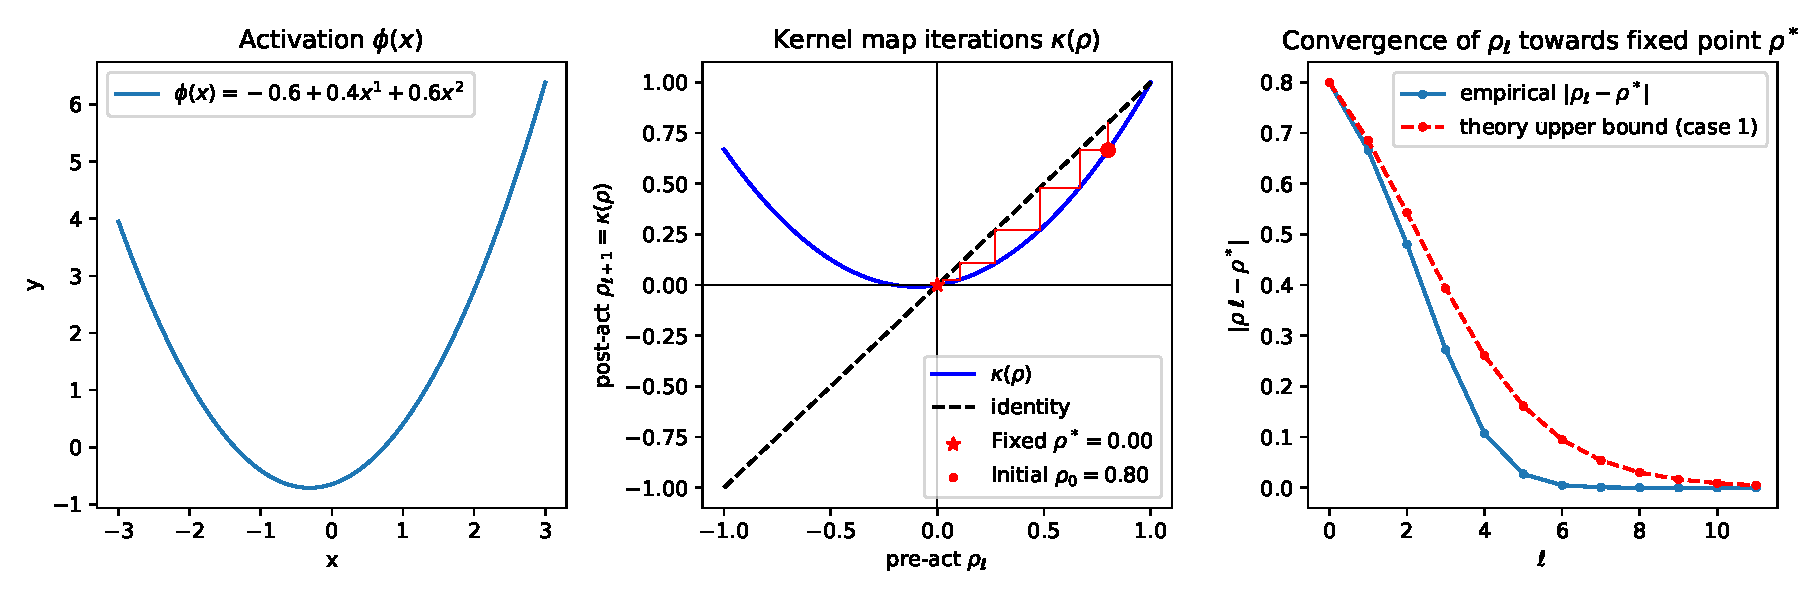
\includegraphics[width=\textwidth]{./kernel_map_convergence_case_0.pdf}
        \caption{\small Case 1}
    \end{subfigure}
    \hfill
    \begin{subfigure}[b]{0.7\textwidth}
        \centering
        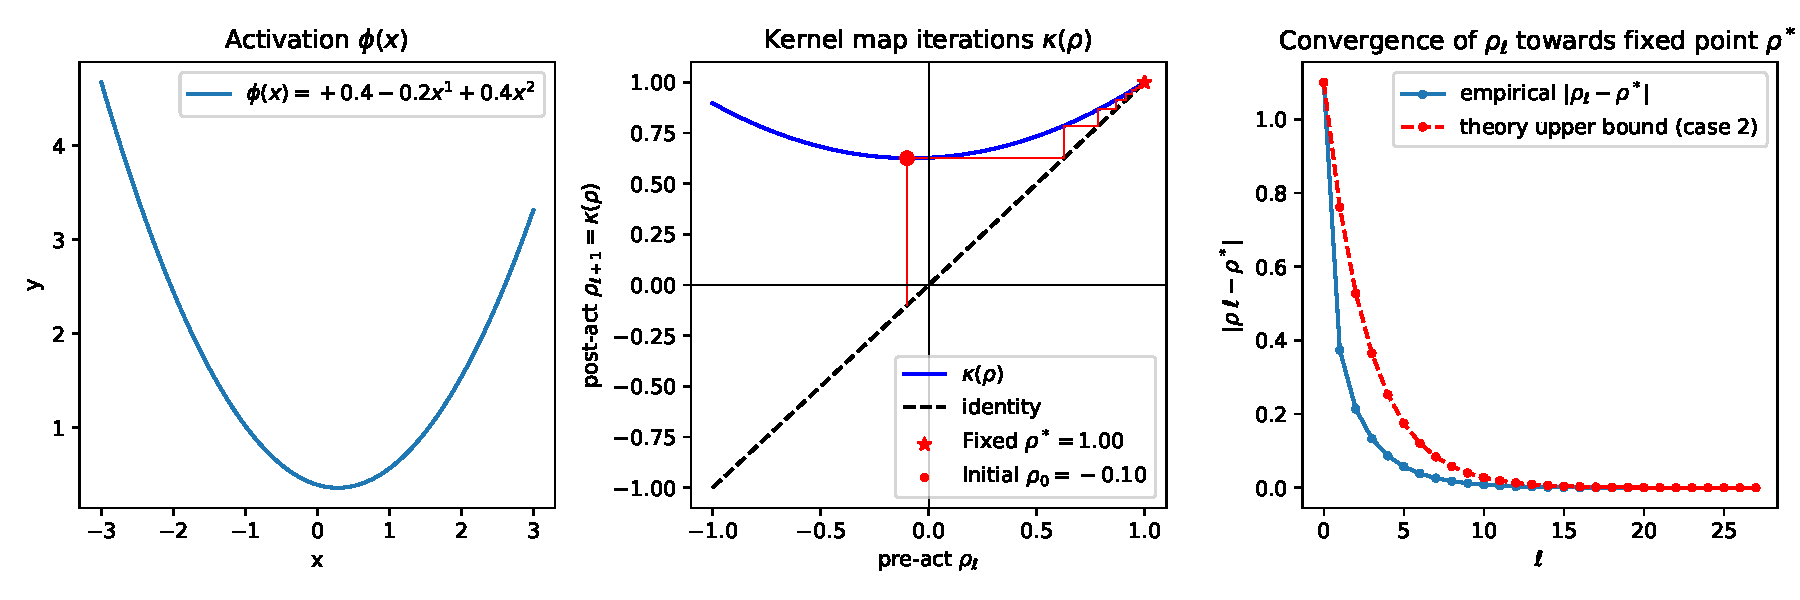
\includegraphics[width=\textwidth]{./kernel_map_convergence_case_1.pdf}
        \caption{\small Case 2}
    \end{subfigure}
    \\
    \begin{subfigure}[b]{0.7\textwidth}
        \centering
        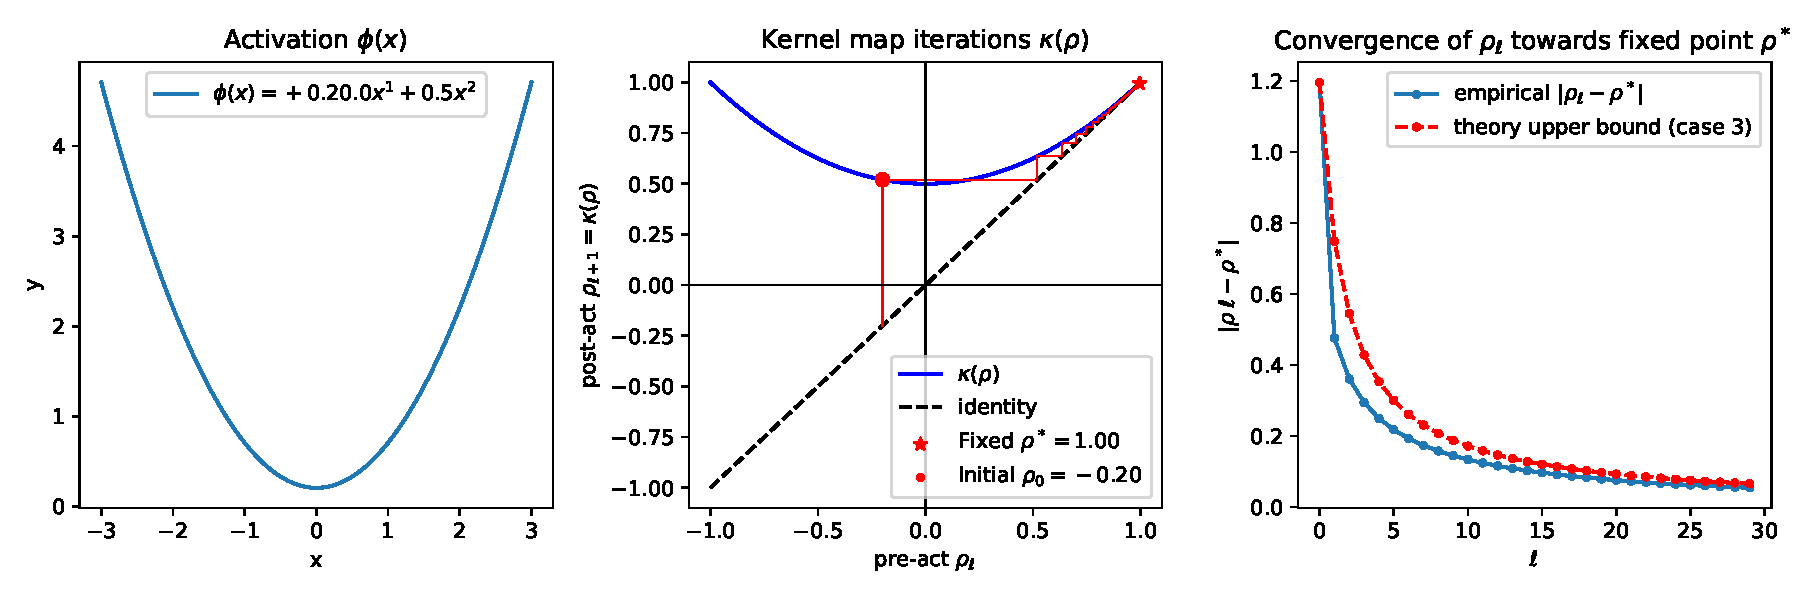
\includegraphics[width=\textwidth]{./kernel_map_convergence_case_2.pdf}
        \caption{\small Case 3}
    \end{subfigure}
    \hfill
    \begin{subfigure}[b]{0.7\textwidth}
        \centering
        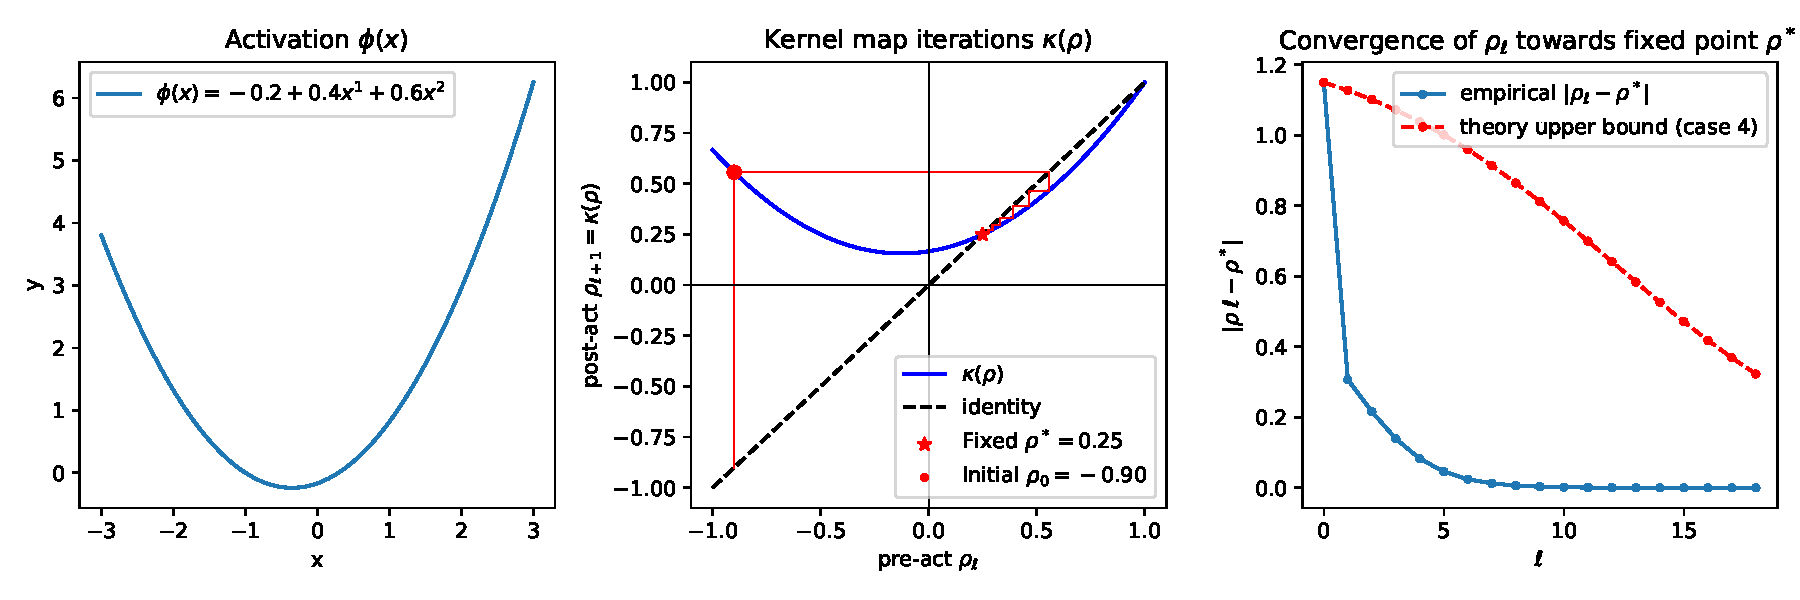
\includegraphics[width=\textwidth]{./kernel_map_convergence_case_3.pdf}
        \caption{\small Case 4}
    \end{subfigure}
    \caption{\small Validation of Theorem~\ref{thm:global_attract}, each corresponding to one of the four cases of the theorem. Left column shows the activation $\phi.$ The middle and right columns show the kernel map show fixed point iteration starting from $\rho_0,$ and applying $\rho_{\ell+1}=\kappa(\rho_\ell)$ for many steps. The middle column shows the kernel map, while the right column shows the distance to the fixed point $\rho^*$.}
    \label{fig:validation_plots}
\end{figure*}

\begin{figure*}[ht!]
    \centering
    \begin{subfigure}[b]{0.7\textwidth}
        \centering
        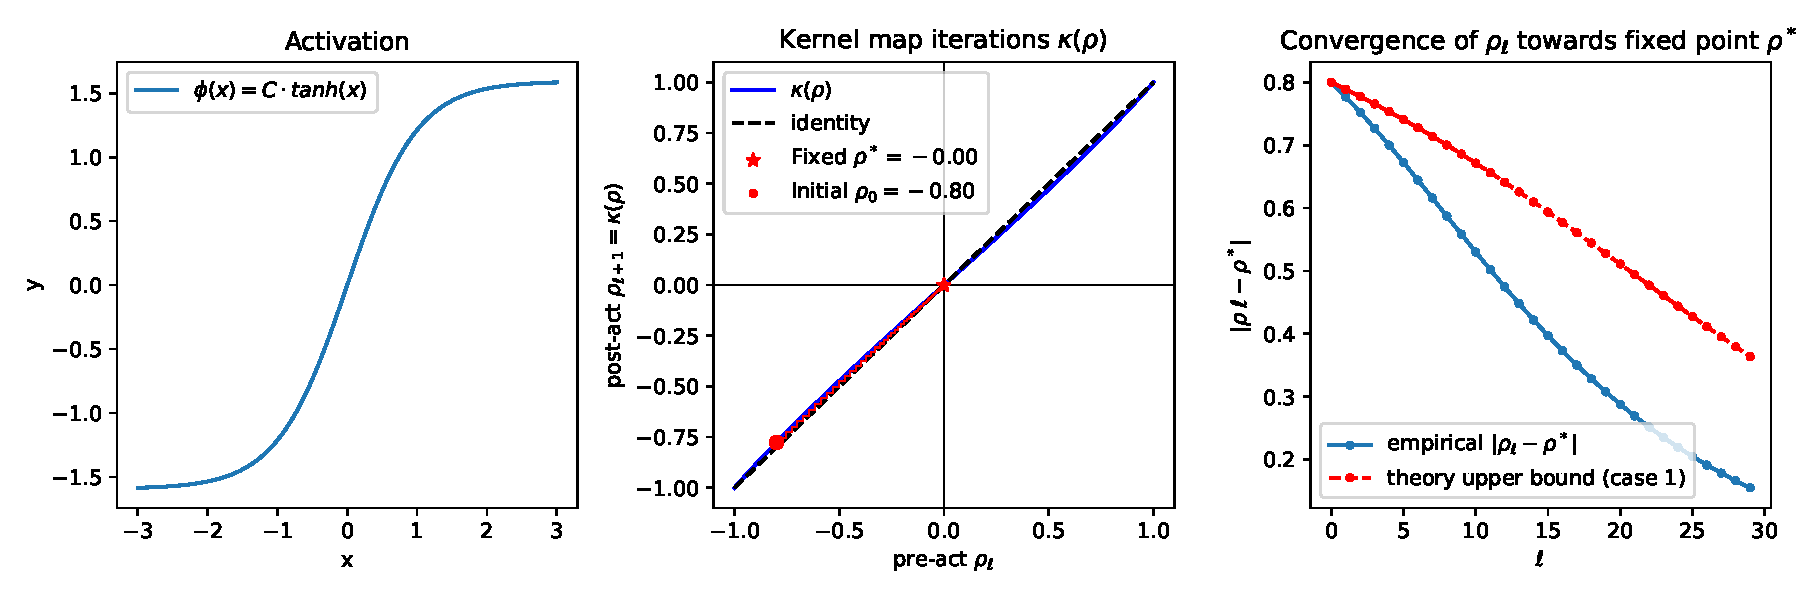
\includegraphics[width=\textwidth]{./kernel_map_convergence_case_0_tanh.pdf}
        \caption{\small Case 1. Tanh activation.}
    \end{subfigure}
    \hfill
    \begin{subfigure}[b]{0.7\textwidth}
        \centering
        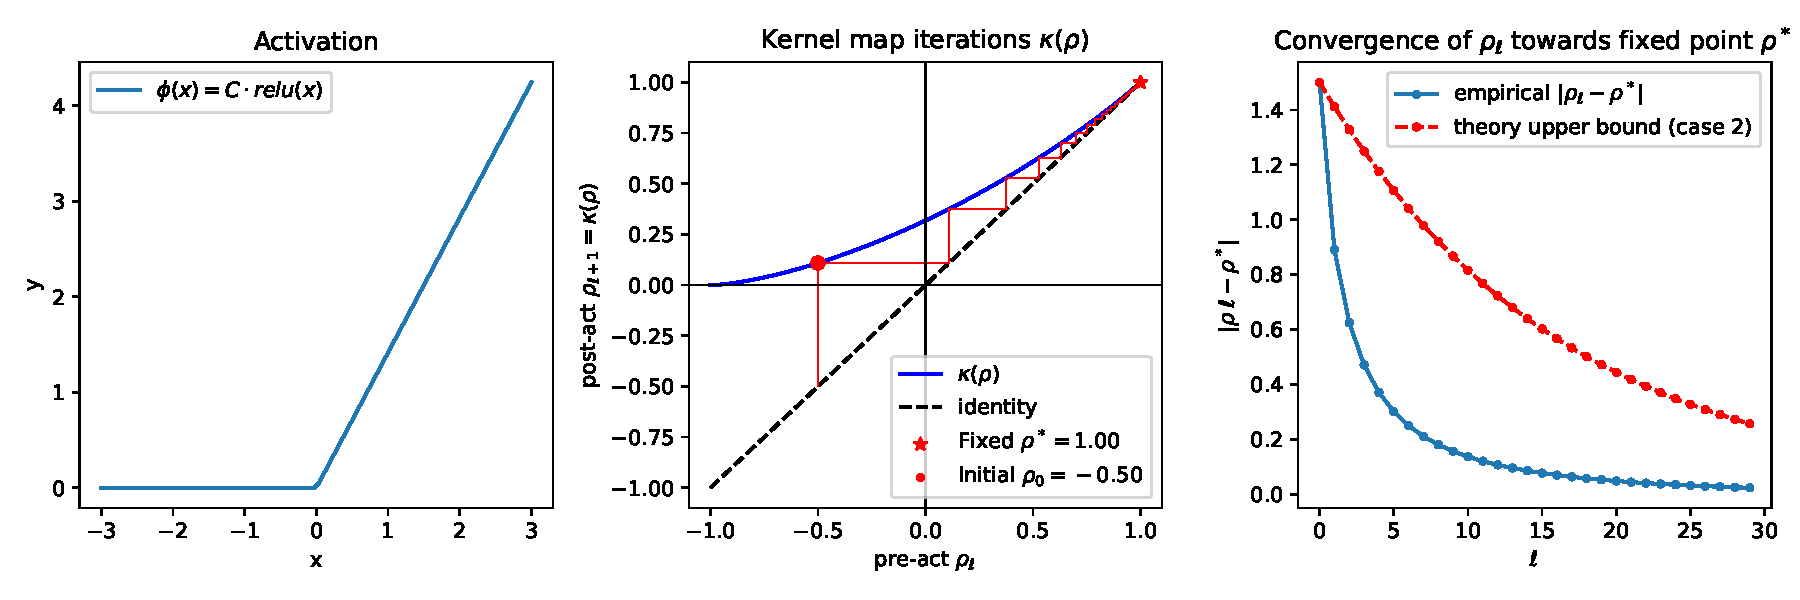
\includegraphics[width=\textwidth]{./kernel_map_convergence_case_1_relu.pdf}
        \caption{\small Case 2: ReLU activation.}
    \end{subfigure}
    \\
    \begin{subfigure}[b]{0.7\textwidth}
        \centering
        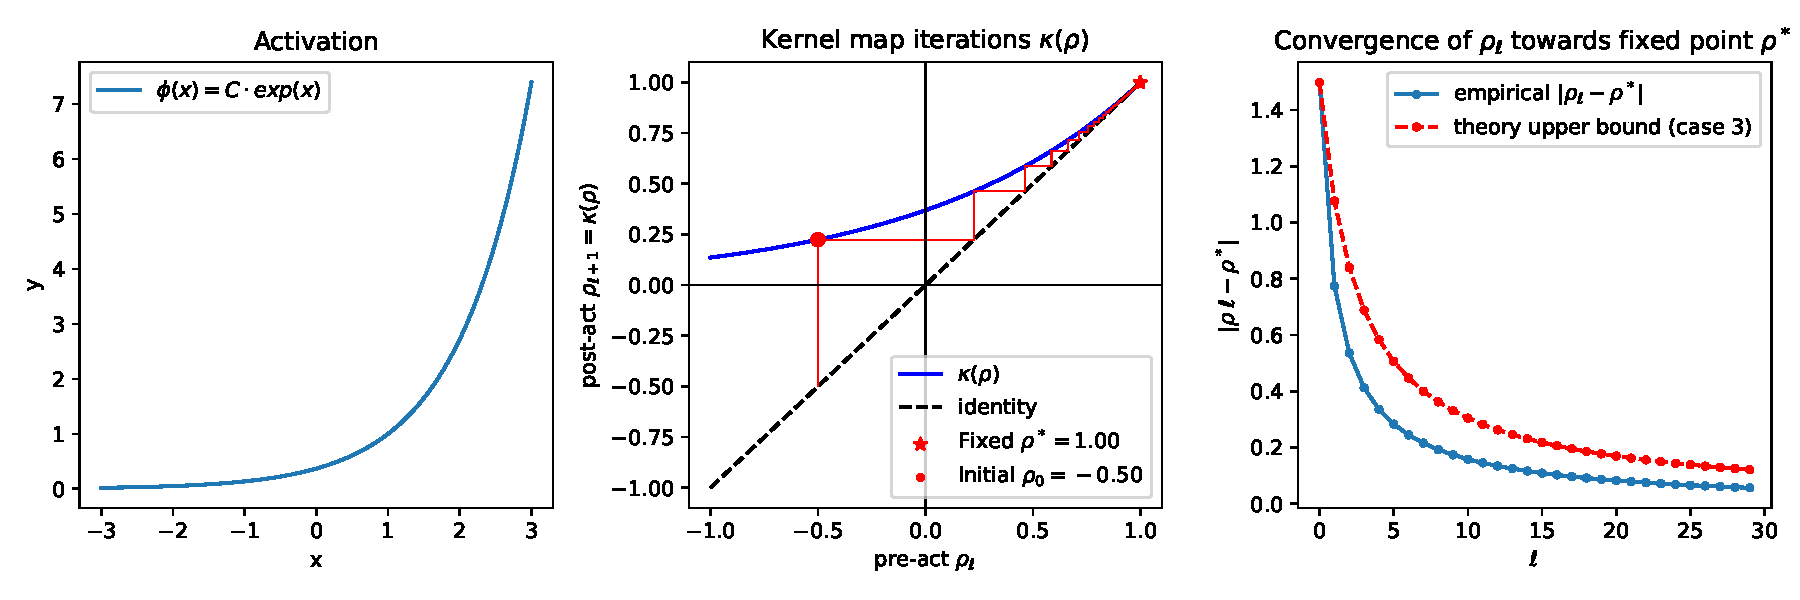
\includegraphics[width=\textwidth]{./kernel_map_convergence_case_2_exp.pdf}
        \caption{\small Case 3: Exponential activation.} 
    \end{subfigure}
    \hfill
    \begin{subfigure}[b]{0.7\textwidth}
        \centering
        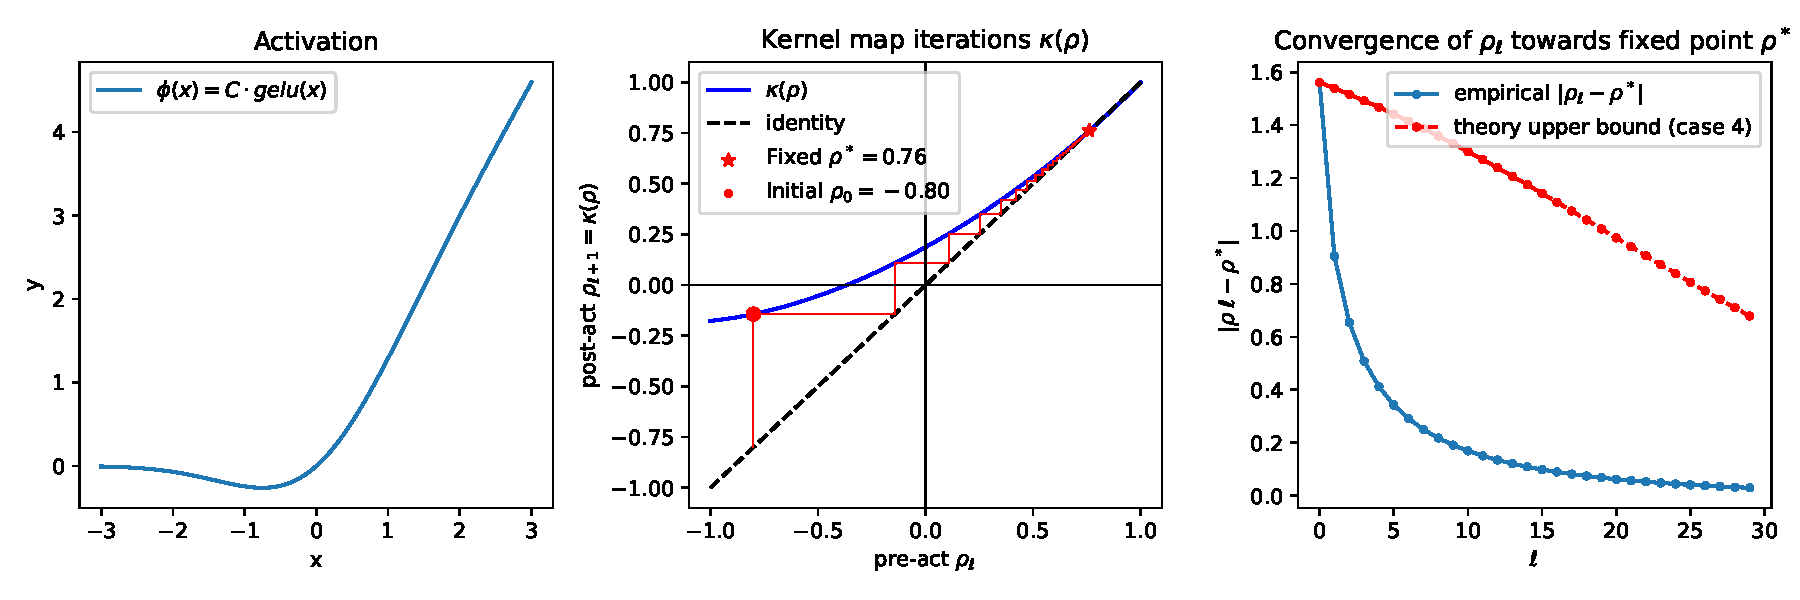
\includegraphics[width=\textwidth]{./kernel_map_convergence_case_3_gelu.pdf}
        \caption{\small Case 4: GELU activation.}
    \end{subfigure}
    \caption{\small Same as Figure~\ref{fig:validation_plots} for some commonly used activations. Note that because the raw activations do not necessarily obey $\E \phi^2(X)=1,$ we have to scale by some constant $C$ to make the activations obey the conditions of the theorem.}
    \label{fig:validation_plots_real_activations}
\end{figure*}

\end{document}
